% ICTAC 25 Talk 

%\documentclass[10pt,xcolor=dvipsnames,xcolor=table,handout]{beamer} 
\documentclass{beamer} 

\title{Testing and Verification of Autonomy\\ with Temporal Constraints}

\author{{\bf Klaus Havelund}, Tracy Clark, Vivek Reddy, Alessandro Pinto\\
Jet Propulsion Laboratory\\
California Institute of Technology\\
%\vspace{1cm}
%{\scriptsize The research was carried out under a contract\\ with the National Aeronautics and Space Administration.}
}

\date[]{JPL - February 4, 2026}



% If you wish to uncover everything in a step-wise fashion, uncomment
% the following command: 
%\beamerdefaultoverlayspecification{<+->}

\mode<presentation>
{ 
\usetheme{Madrid}
\setbeamercovered{transparent=5}
\setbeamertemplate{navigation symbols}{} 
}

\PassOptionsToPackage{bookmarks=true,bookmarksopen=true,pdfborder={0 0 0},pdfhighlight={/N},linkbordercolor=[rgb]{0.5,0.5,0.5},implicit=false,hidelinks}{hyperref}
\usepackage{cite}
\usepackage{amscd}
\usepackage{amsmath,amssymb,amsfonts}
\usepackage{cases}
\usepackage{commath}
\usepackage[hidelinks]{hyperref}
\usepackage{float}
\usepackage{forest}
\usepackage{hhline}
\usepackage{graphicx}

\usepackage{textcomp}
\usepackage{xcolor}
\usepackage{multirow}
\usepackage{tabularx,ragged2e}
\usepackage[skip=2pt]{caption}
\captionsetup[table]{skip=6pt}
\usepackage{subcaption}
\usepackage{multirow}
\usepackage{listings}
\usepackage{xcolor}
\usepackage{todonotes}
\usepackage{rotating}

\usepackage{booktabs} % For better table rules
\usepackage{threeparttable} % For table notes
\usepackage{multirow} % Required for merging rows
\usepackage{tabularx} % For adjustable-width columns
\usepackage{tabto}
\usepackage[most]{tcolorbox}
\usepackage{xcolor}
\usepackage{lipsum}
\usepackage{array}

% table spacing
\setlength{\tabcolsep}{8pt}  % column gap (default is 6pt)
\renewcommand{\arraystretch}{0.95}  % row height (default is 1.0)

\newcommand{\needsref}{\textsuperscript{*}}

\tcbset{
  user/.style={
    colback=blue!5!white,
    colframe=blue!75!black,
    fonttitle=\bfseries,
    title=User,
    sharp corners,
    boxrule=0.5pt,
    left=2mm, right=2mm, top=1mm, bottom=1mm,
  },
  agent/.style={
    colback=gray!10!white,
    colframe=black!60!white,
    fonttitle=\bfseries,
    title=Tool,
    sharp corners,
    boxrule=0.5pt,
    left=2mm, right=2mm, top=1mm, bottom=1mm,
  }
}

\newcommand\ipyt{\lstset{language=python}\lstinline}

\lstdefinestyle{matlab} {
        language=Matlab,
        backgroundcolor=\color[rgb]{0.95,0.95,0.92},
        commentstyle=\color[rgb]{0.13,0.55,0.13}\em,
        stringstyle=\color[rgb]{0.7,0,0},
        basicstyle=\ttfamily\scriptsize}

\lstset{style=matlab,
        captionpos=b,
        frame=single,
        keepspaces=true,
        breakautoindent=true, 
        breakindent=0pt, 
        breaklines=true,
        breakatwhitespace=true,
        numberbychapter=false
        }


\definecolor{backcolour}{rgb}{0.95,0.95,0.92}
\definecolor{codegreen}{rgb}{0,0.6,0}



% style for prompts in the papers sections
\lstdefinestyle{promptPaper}{
        language=Matlab,
        backgroundcolor=\color[rgb]{0.95,0.95,0.92},
        commentstyle=\color[rgb]{0.13,0.55,0.13}\em,
        stringstyle=\color[rgb]{0.7,0,0},
        basicstyle=\ttfamily\scriptsize
}

%json file style
\lstdefinelanguage{json}{
    basicstyle=\ttfamily\scriptsize,
    showstringspaces=false,
    breaklines=true,
    frame=single,
    backgroundcolor=\color[rgb]{0.95,0.95,0.92},
    string=[s]{"}{"},
    morecomment=[l]{:},
    morestring=[b]',
    literate=
     *{0}{{{\color{blue}0}}}{1}
      {1}{{{\color{blue}1}}}{1}
      {2}{{{\color{blue}2}}}{1}
      {3}{{{\color{blue}3}}}{1}
      {4}{{{\color{blue}4}}}{1}
      {5}{{{\color{blue}5}}}{1}
      {6}{{{\color{blue}6}}}{1}
      {7}{{{\color{blue}7}}}{1}
      {8}{{{\color{blue}8}}}{1}
      {9}{{{\color{blue}9}}}{1}
      {:}{{{\color{black}:}}}{1},
}

\def\arrow#1{\stackrel{#1}{\longrightarrow}}
\def\inp#1{^{\bullet}{#1}}
\def\out#1{{#1}^{\bullet}\!}
\def\exec#1{{[#1\rangle}}
\def\prioexec#1{{(#1\rangle}}
\def\free#1{\mathit{free} ( {#1} )}
\def\procs{\Pi}
\def\proc{\pi}
\def\subformula#1{\mathit{sub} (#1)}
\def\Pt{{\cal P}_t}
\def\fab{f_{a\leftrightarrow b}}
\def\avail{\mathit{avail}}
\def\F{\Diamond}
\def\G{\Box}


\def\cl{\mathit{cl}}
\def\arrow#1{\stackrel{#1}{\longrightarrow}}
%\def\best{\mathit{better}}
\def\true{\mathit{true}}
\def\bdd#1{\mathit{BDD}(#1)}
\def\btrue{\mathrm{BDD}(\top)}
\def\bfalse{\mathrm{BDD}(\bot)}
\def\max{\mathrm{BDD}(11\ldots11)}
\def\terms{\tt{terms}}
\def\counting{\mathit{count}}
\def\vars{\mathit{free}}
\def\proj{\mathit{hide}}
\def\ext{\mathit{ext}}
\def\domain{\mathit{domain}}
\def\extend{\mathit{extend}}
\def\lookup{\mathbf{lookup}}
\def\subf{\mathit{sf}}
\def\type{\mathit{type}}
\def\free{\mathit{free}}
\def\bddwedge{\mathbf{and}}
\def\BDDZ#1{\mathrm{BDD0}(#1)}
\def\BDDO#1{\mathrm{BDD1}(#1)}
\def\bddvee{\mathbf{or}}
\def\bddexists{\mathbf{exists}}
\def\bddset{\mathbf{build}}
\def\rename#1#2#3{\mathit{rename} (#1,\,#2,\,#3)}
\def\bddneg{\mathbf{not}}
\def\comp{\mathit{comp}}
\def\old{\mathsf{pre}}
\def\sem{{\cal S}}
\def\current{\mathsf{now}}
\def\nextold{\mathsf{nextpre}}
\def\false{\mathit{false}}
\def\pref#1#2{\mathit{pref}(#1,#2)}
\def\begini#1{\mathit{begin} ( #1 )}
\def\endi#1{\mathit{end} ( #1 )}
\def\maybe{\mathit{maybe}}
\def\pol{\mathit{pol}}
\def\xor{\oplus}
\def\tree#1{\mathit{tree}(#1)}
\def\asgn#1{\mathit{asgn}(#1)}
\def\var#1{\mathit{var}(#1)}
\def\lbl#1{\mathit{lbl}(#1)}
\def\since{\,{\cal S}\,}
\def\sincele#1{{\cal S}_{\leq #1}}
\def\esincele#1{{\cal Z}_{\leq #1}}
\def\sincel#1{{\cal S}_{< #1}}
\def\relle#1{{\cal R}_{\leq #1}}
\def\sinceg#1{{\cal S}_{> #1}}
\def\sincege#1{{\cal S}_{\ge #1}}
\def\relg#1{{\cal R}_{> #1}}
\def\add#1#2{{\mathit{add}(#1,#2)}}
\def\wsince{{\cal S}}
\def\empty{\mathit{empty}}
\def\released{{\cal P}}
\def\LTLsquare{\Box}
\def\BBox{\boxminus}
\def\LTLdiamond{\Diamond}
\def\LTLcircle{{\bigcirc}}
\def\GI{{\textfrak{I}}}
\def\SSI{{\textswab{I}}}
\newcommand\lola{\textsc{Lola}}
\newcommand\B{{\mathbb B}}
\newcommand\AP{\mathit{AP}}
\newcommand\buchi{B\"uchi}
\newcommand\cla{\mathsf{cone}}
\newcommand\sla{\mathsf{sla}}
\newcommand\suc{\mathsf{suc}}
\newcommand\clr{\mathsf{clr}}
\newcommand\cobuchi{Co-B\"uchi}
\newcommand\frag{\mathsf{frag}}
\newcommand\res{\mathsf{res}}
\newcommand\safe{\mathsf{safe}}
\newcommand\tempt{\mathsf{tempt}}
\newcommand\opt{\textrm{opt}}
\newcommand\best{\textrm{best}}
\newcommand\worst{\textrm{worst}}

%%%%%%%%%%%%%%%%
% Mathematics: %
%%%%%%%%%%%%%%%%

\newcommand{\boolty}{\mathbb{B}}

%%%%%%%%%%%%
% Symbols: %
%%%%%%%%%%%%

\newcommand\event[2]{{\em #1}(\text{#2})}
\newcommand\eventname[1]{{\em #1}}
\newcommand\args[1]{\text{#1}}
\newcommand{\symb}[1]{`$#1$'}
\newcommand{\seen}[1]{\mathit{}{seen}(#1)}
\newcommand{\alreadyseen}[1]{\mathit{}{\Theta}(#1)}

\newcommand\kwif{{\bf if\ }}
\newcommand\kwthen{{\bf then\ }}
\newcommand\kwelse{{\bf else\ }}

\newcommand\id[1]{\mathit{#1}}

\newcommand\DiamondMinus{\ensurestackMath{%
  \stackengine{.8pt}{\Diamond}{\scalebox{.65}[1.15]{$-$}}{2}{c}{F}{F}{L}}}

%%%%
\def\MnSymbolGlyphs#1{% IF ONE NEEDS TO LOCATE GLYPHS
  \usepackage{MnSymbol,fonttable}%
  \AtBeginDocument{\fonttable{MnSymbol#110}}%
}

\def\ImportFromMnSymbol#1{%
  \DeclareFontFamily{U} {MnSymbol#1}{}
  \DeclareFontShape{U}{MnSymbol#1}{m}{n}{
   <-6> MnSymbol#15
   <6-7> MnSymbol#16
   <7-8> MnSymbol#17
   <8-9> MnSymbol#18
   <9-10> MnSymbol#19
   <10-12> MnSymbol#110
   <12-> MnSymbol#112}{}
  \DeclareFontShape{U}{MnSymbol#1}{b}{n}{
   <-6> MnSymbol#1-Bold5
   <6-7> MnSymbol#1-Bold6
   <7-8> MnSymbol#1-Bold7
   <8-9> MnSymbol#1-Bold8
   <9-10> MnSymbol#1-Bold9
   <10-12> MnSymbol#1-Bold10
   <12-> MnSymbol#1-Bold12}{}
  \DeclareSymbolFont{MnSy#1} {U} {MnSymbol#1}{m}{n}
}
\newcommand\DeclareMnSymbol[4]{\DeclareMathSymbol{#1}{#2}{MnSy#3}{#4}}
% %%%%
\ImportFromMnSymbol{C}
\DeclareMnSymbol{\DDiamond}{\mathrel}{C}{120}

\renewcommand{\baselinestretch}{0.957}

% Klaus's macros

\usepackage{graphicx}
\usepackage{relsize}
\usepackage{stmaryrd}
\usepackage{algorithm}
\usepackage{algpseudocode}
\newcommand\matl{{\sf MaTL}}
\newcommand\para[1]{\vspace{2ex}\noindent{\bf #1.}}
\newcommand\subpara[1]{\underline{{\em #1.}}}
\newcommand{\Next}{\mathbin{\scalebox{0.8}{$\bigcirc$}}}
\newcommand{\prev}{\ominus}
\def\until{\;{\cal U}\;}
\def\wuntil{\;{\cal U_{\text{w}}}\;}
\def\wsince{\;{\cal S_{\text{w}}}\;}
\def\wnext{\,{\cal \Next_{\text{w}}}\,}
\def\wprev{\,{\cal \prev_{\text{w}}}\,}
\newcommand\ignore[1]{}
\renewcommand\true{\tt{tt}}
\renewcommand\false{\tt{ff}}
\renewcommand\iff{{\bf iff}}
\newcommand{\tabconst}{3.3cm}
\newcommand{\tabconste}{3.8cm}

\newcommand{\match}[3]{\mathsf{Match}\llbracket#1\rrbracket\left(#2\right)\left(#3\right)}
\newcommand{\pat}[3]{\mathsf{Pat}\llbracket#1\rrbracket\left(#2\right)\left(#3\right)}
\renewcommand{\eval}[2]{\mathsf{Eval}\llbracket#1\rrbracket\left(#2\right)}
\newcommand{\oper}[3]{\mathsf{Op}\llbracket#1\rrbracket\left(#2,\,#3\right)}
\newcommand{\rel}[3]{\mathsf{Rel}\llbracket#1\rrbracket\left(#2,\,#3\right)}
\newcommand{\reg}[2]{\mathsf{Reg}\llbracket#1\rrbracket\left(#2\right)}

\newcommand\nat{\mathbb{N}}
\newcommand\intg{\mathbb{Z}}
\newcommand\bool{\mathbb{B}}

\newcommand\fuzz{{\tt fuzz}}
\newcommand\sut{{\tt SUT}}

\definecolor{literalcolor}{rgb}{1,0,1}      % Pink for literals
\definecolor{operatorcolor}{rgb}{0,0.5,0.5} % Teal for operators (consistent with DejaVu)

\lstdefinelanguage{fuzzdsl}{
    keywords={
        rule, not, or, and, always, eventually, until, wuntil, next, wnext, sofar, once, since, wsince, prev, wprev, count, countpast, matches, any
    },
    literate=
        {|-}{{{\color{operatorcolor}$\vdash$}}}1
        {>}{{{\color{operatorcolor}$>$}}}1
        {<}{{{\color{operatorcolor}$<$}}}1
        {=}{{{\color{operatorcolor}$=$}}}2
        {>=}{{{\color{operatorcolor}$\ge$}}}1
        {<=}{{{\color{operatorcolor}$\le$}}}1
        {=>}{{{\color{red}$\Rightarrow$}}}1
        {[}{{{\color{red}$[$}}}1
        {]}{{{\color{red}$]$}}}1
        {<<}{{{\color{red}$<$}}}1
        {>>}{{{\color{red}$>$}}}1
        {+}{{{\color{operatorcolor}$+$}}}1
        {-}{{{\color{operatorcolor}$-$}}}1
        {*}{{{\color{operatorcolor}$*$}}}1
        {/}{{{\color{operatorcolor}$/$}}}1
        ,
    morecomment=[l]{\#},  
    backgroundcolor=\color{white},   
    commentstyle=\color{codegreen},
    keywordstyle=\color{blue},
    basicstyle=\ttfamily\scriptsize,
    breakatwhitespace=false,         
    breaklines=true,                 
    keepspaces=true,                      
    numbersep=5pt,                  
    showspaces=false,                
    showstringspaces=false,
    showtabs=false,                  
    tabsize=2,
    aboveskip=5pt,
    belowskip=2pt,
    frame=tblr,
    aboveskip=1em,    
    belowskip=1em,    
}

\newcommand{\fuzzdsl}{\lstset{language=fuzzdsl,backgroundcolor=\color{white}, frame=none}}
\newcommand{\ifuzz}{\fuzzdsl\lstinline}

\lstset{
  aboveskip=1em,    % space before each listing
  belowskip=1em,    % space after each listing
  basicstyle=\ttfamily\small,  % example style
  frame=single,     % optional: adds a frame around the listing
}

%\newcommand{\conjarrow}{\mathrel{\&\!\!\!\!\rightarrow}}

\lstset{
%  basicstyle=\ttfamily,
%  columns=fullflexible,
columns=fullflexible,keepspaces,
%    numberstyle=\tiny,
showstringspaces=false, % otherwise not possible to copy and paste
%        aboveskip=-40pt,
%        frame=leftline
% numbers=left,
  frame=single,
  language=Scala,
%  basicstyle=\small\ttfamily,
  basicstyle=\scriptsize\ttfamily,
  keywordstyle=\bfseries\color{red!60!blue},
  commentstyle=\ttfamily\color{tuggreen},
  stringstyle=\color{blue},
  backgroundcolor=\color{gray!10!white},
 morekeywords=[2]{1, 2, 3, 4, 5, 6, 7, 8, 9, 0},
  keywordstyle=[2]{\color{blue!20!pink}},
%  numberstyle=\tiny\color{gray},
%  emphlines={7},emphstyle=\color{tugred}
%  backgroundcolor=\color{yellow}
}

\lstdefinelanguage{tasknetdsl}{
    keywords={
        tasknet, 
        end, 
        timelines, 
        atomic,
        state,
        cumulative,
        bounds,
        rate,
        taskdef,
        pre,
        inv,
        maint,
        post,
        in,
        impacts,
        optional,
        task,
        durationrange,
        startrange,
        endrange,
        after,
        containedin,
        constraints,
        properties,
        prop,
        not,
        and,
        implies,
        or,
        always,
        eventually,
        until,
        sofar,
        once,
        since
    },
    literate=
        {|-}{{{\color{operatorcolor}$\vdash$}}}1
        {>}{{{\color{operatorcolor}$>$}}}1
        {<}{{{\color{operatorcolor}$<$}}}1
        {=}{{{\color{operatorcolor}$=$}}}2
        {>=}{{{\color{operatorcolor}$\ge$}}}1
        {<=}{{{\color{operatorcolor}$\le$}}}1
        {=>}{{{\color{red}$\Rightarrow$}}}1
        {[}{{{\color{red}$[$}}}1
        {]}{{{\color{red}$]$}}}1
        {<<}{{{\color{red}$<$}}}1
        {>>}{{{\color{red}$>$}}}1
        {+}{{{\color{operatorcolor}$+$}}}1
        {-}{{{\color{operatorcolor}$-$}}}1
        {*}{{{\color{operatorcolor}$*$}}}1
        {/}{{{\color{operatorcolor}$/$}}}1
        ,
    morecomment=[l]{\#},  
    backgroundcolor=\color{white},   
    commentstyle=\color{codegreen},
    keywordstyle=\color{blue},
    basicstyle=\ttfamily\scriptsize,
    breakatwhitespace=false,         
    breaklines=true,                 
    keepspaces=true,                      
    numbersep=5pt,                  
    showspaces=false,                
    showstringspaces=false,
    showtabs=false,                  
    tabsize=2,
    aboveskip=5pt,
    belowskip=2pt,
    frame=tblr,
    aboveskip=1em,    
    belowskip=1em,    
}

\newcommand{\tasknetdsl}{\lstset{language=tasknetdsl,backgroundcolor=\color{white}, frame=none}}
\newcommand{\itasknet}{\tasknetdsl\lstinline}

% ===\

%\ignore{
\setbeamertemplate{footline}{%
  \leavevmode%
  \hbox{%
    \begin{beamercolorbox}[wd=\paperwidth,ht=1.6ex,dp=0.2ex,leftskip=0.6em,rightskip=0.6em]{author in head/foot}%
      \usebeamerfont{author in head/foot}%
      \fontsize{5}{5}\selectfont \copyright 2026. 
      All rights reserved. This document has been reviewed and the information being released does not contain export controlled technical data%
      \hfill%
      \fontsize{5}{5}\selectfont \insertframenumber/\inserttotalframenumber%
    \end{beamercolorbox}%
  }%
}
%}

% ===/

\newcommand{\conjarrow}{\mathrel{\&\!\!\!\!\rightarrow}}

\begin{document}

\begin{frame}
  \titlepage
\end{frame}


%----------------------------------------
\begin{frame}
  \frametitle{Placing numbers in a sequence of trays}\small
  \centering
  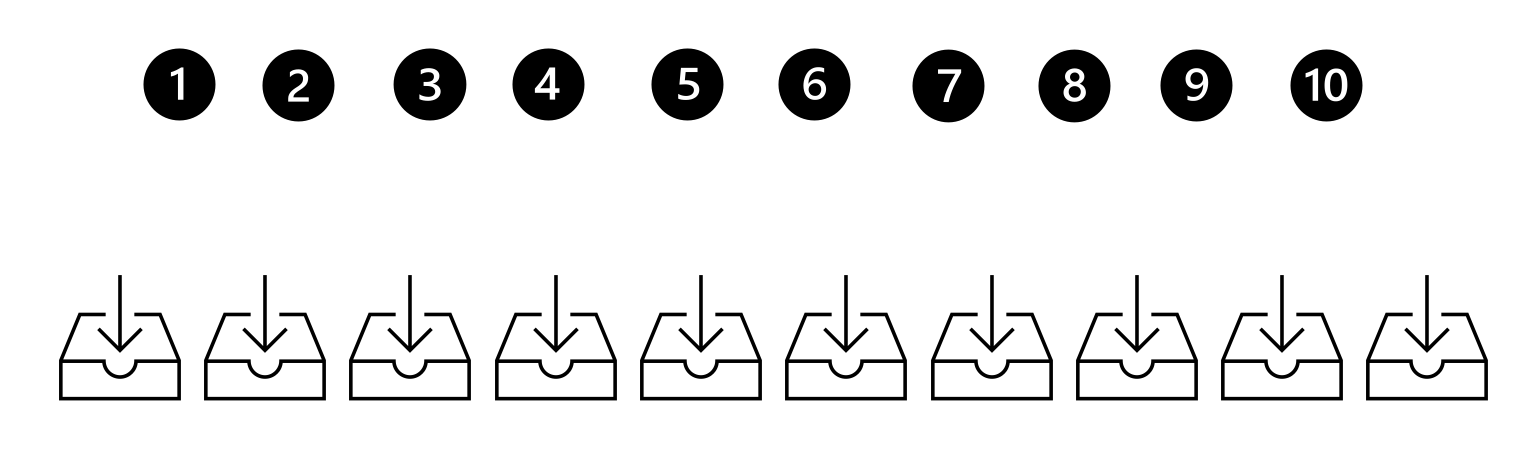
\includegraphics[width=\textwidth]{figures/balls.png}

  \begin{block}{}\scriptsize
    \begin{itemize}
    \item After 2 should eventually follow 6.   
    \item After 7 all numbers should be bigger than 7.
    \item A 1 should be preceded in the past by  a 3.
  \end{itemize}
\end{block}

\end{frame}

%----------------------------------------
\begin{frame}
  \vspace{1.2cm}

  \frametitle{Placing numbers in a sequence of trays}\small
  \centering
  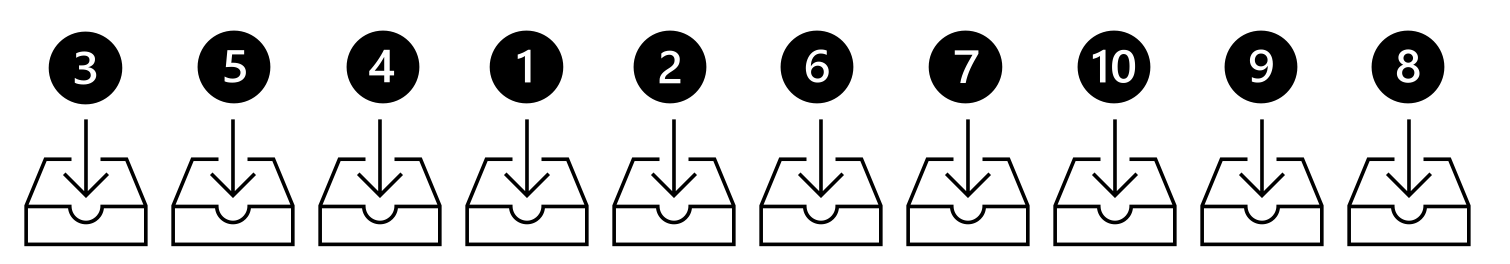
\includegraphics[width=\textwidth]{figures/balls-assigned.png}

  \vspace{0.3cm}

  \begin{block}{}\scriptsize
    \begin{itemize}
    \item After 2 should eventually follow 6.   
    \item After 7 all numbers should be bigger than 7.
    \item A 1 should be preceded in the past by  a 3.
  \end{itemize}
\end{block}
  
\end{frame}

%----------------------------------------
\begin{frame}[fragile]
  \frametitle{Modeling temporal logic in first-order logic on a finite trace} \small

\begin{block}{Consider the first temporal property}\scriptsize
\begin{itemize}
\item After 2 should eventually follow 6. 
\end{itemize}

\[
\Box (2 \rightarrow \Diamond 6)
\]

\begin{lstlisting}[language=tasknetdsl,frame=single]
                        always (2 implies eventually 6);
\end{lstlisting}

\end{block}

\pause

\vspace{0.2cm}
{\bf It can be translated to a first-order logic formula constraining $tray$:}

\[
\forall i \in \{1..k\},\ tray(i) = 2 
  \rightarrow 
    \exists j \in \{i..k\}, tray(j) = 6
\]

\pause

\vspace{0.2cm}
{\bf Then we can ask an SMT solver such as Z3\\ 
\url{https://github.com/Z3Prover/z3}\\ 
to find an assignment of numbers to trays positions that satisfies this formula.}

\end{frame}
%----------------------------------------
\begin{frame}[fragile]
  \frametitle{First application}

{\Large\bf Using Temporal Constraints to Generate Tests}

\end{frame}

%----------------------------------------
\begin{frame}
  \frametitle{Command driven systems} \small

\begin{figure}
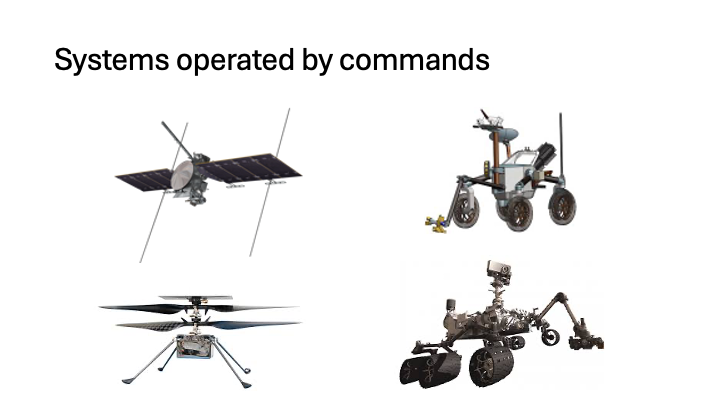
\includegraphics[width=1.0\textwidth]{figures/start1.png}
%\caption{Your caption}
\end{figure}

\begin{block}{}\scriptsize
The system is operated by commands being submitted to it.  
\end{block}

\end{frame}


%----------------------------------------
\begin{frame}
  \frametitle{Command driven system} \small

\begin{figure}
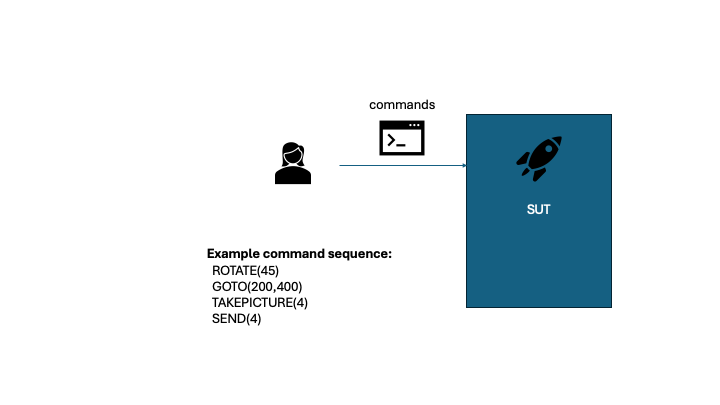
\includegraphics[width=1.0\textwidth]{figures/start2.png}
%\caption{Your caption}
\end{figure}

\begin{block}{}\scriptsize
Command driven systems of interest are those operated by sequences of commands.  
\end{block}

\end{frame}


%----------------------------------------
\begin{frame}
  \frametitle{Command driven system under test} \small

\begin{figure}
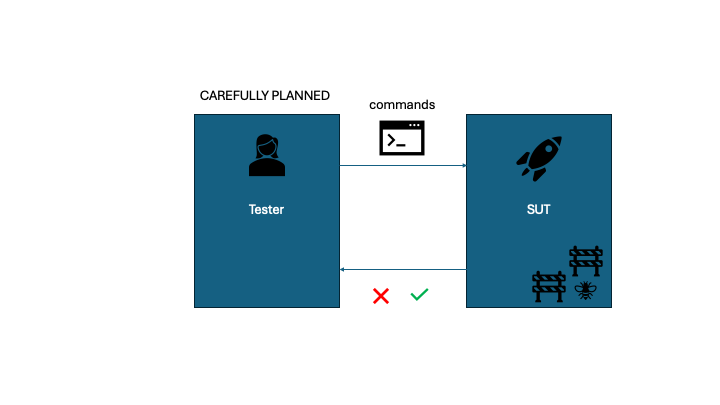
\includegraphics[width=1.0\textwidth]{figures/start3.png}
%\caption{Your caption}
\end{figure}

\begin{block}{}\scriptsize
Traditionally such a system is tested by manual creation of carefully planned command sequences.
\end{block}

\end{frame}


%----------------------------------------
\begin{frame}
  \frametitle{Command driven system under test} \small

\begin{figure}
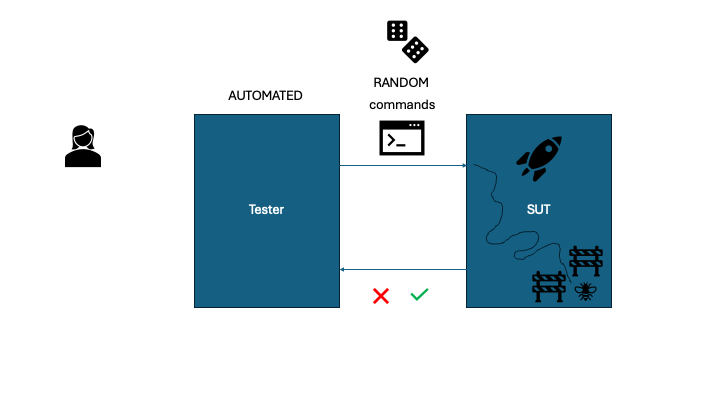
\includegraphics[width=1.0\textwidth]{figures/start4.png}
%\caption{Your caption}
\end{figure}

\begin{block}{}\scriptsize
However, this may not get into the corners of the SUT. We therefore want to fuzz test the SUT by sending random commands to it. But not too random, we want to constrain the randomness.
\end{block}

\end{frame}


%----------------------------------------
\begin{frame}
  \frametitle{Command driven system under test} \small

\begin{figure}
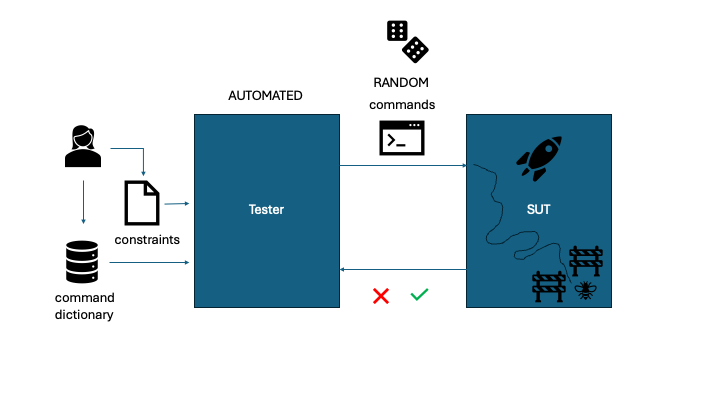
\includegraphics[width=1.0\textwidth]{figures/start5.png}
%\caption{Your caption}
\end{figure}

\begin{block}{}\scriptsize
The user defines what commands are possible and constraints on the randomness using an expressive
temporal logic.
\end{block}

\end{frame}


%----------------------------------------
\begin{frame}<0>
  \frametitle{Plan as a T-diagram} \small

\begin{figure}
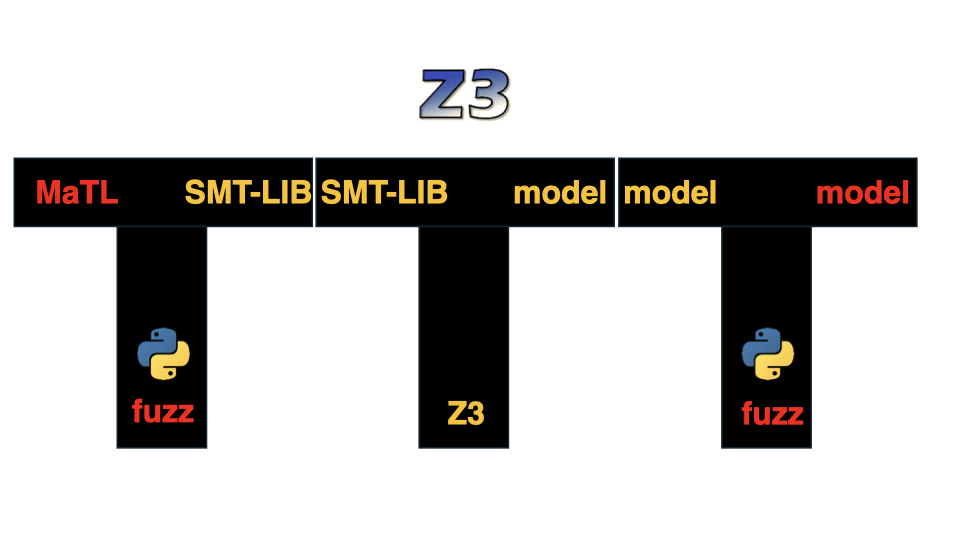
\includegraphics[width=0.8\textwidth]{figures/t-diagram.png}
%\caption{Your caption}
\end{figure}

\begin{block}{}\scriptsize
Our main tasks: 

\begin{enumerate}

\item Design the MaTL temporal logic.
\item Develop translator from MaTL to SMT-LIB. 
\item Refine (further randomize) model generated by Z3.

\end{enumerate}

\end{block}

\end{frame}
  

%----------------------------------------
\begin{frame}[fragile]
  \frametitle{Commands and tests} \small

\begin{definition}[Command]
A command is a dictionary mapping command name and arguments:

\begin{lstlisting}[language=python,frame=single]
Command = Dict[str, Union[int, float, str]]
\end{lstlisting}
\end{definition}

Example of command $goto(x=100,y=200)$:

\[
["name" : "goto", "x": 100, "y": 200]
\]

\pause
\begin{definition}[Test]
A test is a list of commands

\begin{lstlisting}[language=python,frame=single]
Test = list[Command]
\end{lstlisting}
\end{definition}

\end{frame}

%----------------------------------------
\begin{frame}<0>{Hidden slide}
  \frametitle{Matching Temporal Logic (MaTL) - the match construct} \small

Consider the trace:

\[ 
[ 
open(file=\texttt{"log"}, mode=\texttt{"r"}),
read(file=\texttt{"log"}),
close(file=\texttt{"log"})
]
\]

\pause

\begin{block}{We want a formula of the form}
\begin{equation*}
\begin{aligned}
\varphi \;::=&\; ...  \;|\; \langle id(m) \rangle \varphi \;|\; ...
\end{aligned}
\end{equation*}
\end{block}

\pause

\vspace{0.2cm}

For example, at the first trace position the following formula is true,
\underline{binding $f$ to $\texttt{"log"}$},
if $\varphi$ thereafter is true in scope of this binding:

\[
\langle open(file=f?, mode="r") \rangle \varphi
\]

\pause

\vspace{0.2cm}

At the last position the following formula is true, \underline{assuming $f$ is in scope} and denotes $\texttt{"log"}$), if $\varphi$ is thereafter true:

\[
\langle close(file=f) \rangle \varphi
\]

\end{frame}

%----------------------------------------

\begin{frame}<0>
  \frametitle{A test is a list of commands} \small

\begin{block}{Property}\scriptsize
If at some position in the test there is a MOVE command with a distance `$d$’, then later there must be a ROTATE command
with an angle `$a$’ such that the predicate $P(d,a)$ holds.
\end{block}

\begin{figure}
\includegraphics[width=1.0\textwidth]{figures/slide1.png}
%\caption{Your caption}
\end{figure}

\begin{block}{}\scriptsize
A test is a sequence of commands. A test
can satisfy a temporal property or not.
\end{block}

\end{frame}

%----------------------------------------
\begin{frame}<0>
  \frametitle{MaTL syntax} \small

\begin{equation*}
\begin{aligned}
\varphi \;::=&\; \true 
  \;|\; \neg \varphi 
  \;|\; \varphi_1 \lor \varphi_2 \pause
  \;|\; \langle id(m) \rangle \varphi \pause
  \;|\; e_1 \; \diamond \; e_2 
  \;|\; e \vdash r \\[0.5ex] \pause
    & \Next \varphi 
  \;|\; \varphi_1 \until \varphi_2 
  \;|\; \prev \varphi 
  \;|\; \varphi_1 \since \varphi_2 \pause
  \;|\; \Sigma^{+}_{[a,b]} \varphi 
  \;|\; \Sigma^{-}_{[a,b]} \varphi \\[0.5ex] \pause \\
m \;::=&\; \epsilon \;|\; m_1 \; m_2 \;|\; id = p \\[0.5ex]
p \;::=&\; x? \;|\; x \;|\; c \;|\; id_1.id_2 \\[0.5ex] \pause \\
e \;::=&\; x \;|\; c \;|\; id_1.id_2 \;|\; e_1 \; \otimes \; e_2 \\[0.5ex]
\diamond \;::=&\; < \;|\; \le \;|\; = \;|\; \neq \;|\; \ge \;|\; > \\[0.5ex]
\otimes \;::=&\; + \;|\; - \;|\; \times \;|\; \div 
\end{aligned}
\end{equation*}

\end{frame}


%----------------------------------------
\begin{frame}<0>
  \frametitle{Example} \small

\begin{block}{Requirement}
Whenever a file f is opened, it is eventually closed.
\end{block}

What we can write using the core syntax:

\[
\neg (\true \until (\langle open(file=f?)\rangle \neg(\true \until close(file=f))))
\]

\pause

We might instead want to to write:

%\[
%\Box ( [ open(file=f?) ] \Diamond close(file=f))
%\]

%\pause

%Or even:

\[
\Box (open(file=f?) \Rightarrow \Diamond close(file=f))
\]

\vspace{0.2cm}

% The latter two forms are derived syntax.

The last form is {\bf derived} syntax.

\end{frame}


%----------------------------------------
\begin{frame}<0>
  \frametitle{Derived syntax} \small

\[
\begin{array}{rcl@{\hspace{2em}}ll}

\false & = & \neg \true                     & \text{false} & (1)\\

\varphi_1 \wedge \varphi_2 &=& \neg(\neg \varphi_1 \vee \neg \varphi_2) & \text{and} & (2)  \\

\varphi_1 \rightarrow \varphi_2 &=& \neg \varphi_1 \vee \varphi_2       & \text{implication} & (3) \\

%e_1 \diamond_1 e_2 \diamond_2 e_3 &=& e_1 \diamond_1 e_2 \wedge e_2 \diamond_2 e_3 & \text{ternary relation} & (4)\\ 

\\

%\pause

[id(m)] \varphi &=& \neg \langle id(m) \rangle \neg \varphi & \text{universal modality} & (5)\\ 

%\pause

%id(m) \Rightarrow  \varphi &=& [id(m)] \varphi & \text{universal modality} & (6)\\

%\pause

%id(m) \bullet \varphi &=& \langle id(m) \rangle \varphi & \text{existential modality} & (7)\\

%\pause

id(m) &=& \langle id(m) \rangle \true      & \text{event occurrence} & (8)\\

\\

%\pause

\Diamond \varphi &=& \true \until \varphi & \text{eventually in the future} & (9)\\

\Box \varphi &=& \neg \Diamond \neg \varphi & \text{always in the future} & (10)\\

\DDiamond \varphi &=& \true \since \varphi & \text{sometime in the past} & (11)\\

\BBox \varphi &=& \neg \DDiamond \neg \varphi & \text{always in the past} & (12)\\ \\

\varphi_1 \wuntil \varphi_2 &=& (\varphi_1 \until \varphi_2) \vee \Box \varphi_1 & \text{weak until} & (13)\\

\varphi_1 \wsince \varphi_2 &=& (\varphi_1 \since \varphi_2) \vee \BBox \varphi_1 & \text{weak since} & (14)\\

\wnext \varphi &=& \next \varphi \vee \neg \next \true & \text{weak next} & (15)\\

\wprev \varphi &=& \prev \varphi \vee \neg \prev \true & \text{weak previous} & (16)\\

\end{array}
\]

\end{frame}


%----------------------------------------
\begin{frame}<0>
  \frametitle{Derived syntax} \small

\[
\begin{array}{rcl@{\hspace{2em}}ll}

\Sigma^{+}_{a} \varphi  &=& \Sigma^{+}_{[a,a]} \varphi & \text{future exact count} & (17)\\

\Sigma^{-}_{a} \varphi &=& \Sigma^{-}_{[a,a]} \varphi & \text{past exact count} & (18)\\

%\pause

\Next_a \varphi &=& \Next \Next ... \Next  \varphi  \quad (\text{a times}) & \text{a steps in future} & (19)\\

\prev_a \varphi &=& \prev \prev ... \prev \varphi \quad (\text{a times}) & \text{a steps in past} & (20)\\

\end{array}
\]

\end{frame}


%----------------------------------------
\begin{frame}<0>
  \frametitle{A small file example} \small

An example trace:

\[ 
[
open(file=\texttt{"log"}, mode=\texttt{"r"}),
read(file=\texttt{"log"}),
close(file=\texttt{"log"})
]
\]

\pause

\begin{block}{Requirement}
(1) Whenever a file $f$ is opened, it is eventually closed.\\
(2) Whenever a file $f$ is read from, in the past it has been opened in read mode, and not closed since.\\
(3) There should be one open event in read mode.
\end{block}

\pause

\begin{equation*}
\begin{aligned}
(1) \;&\; \Box (open(file=f?) \Rightarrow \Diamond close(file=f)) \\[0.5ex]
(2) \;&\; \Box (read(file=f?) \Rightarrow \neg close(file=f) \since open(file=f, mode=\texttt{"r"}) \\[0.5ex]
(3) \;&\; \Sigma^{+}_1 open(mode=\texttt{"r"})
\end{aligned}
\end{equation*}

\end{frame}


%
%----------------------------------------
\begin{frame}
  \frametitle{Semantics} \small

\begin{definition}[Assignments]

An assignment is a mapping from command field names to values:

\[
\gamma \in \Gamma = X \stackrel{m}{\rightarrow} V
\]

\begin{itemize}
    \item $\epsilon$ denotes the empty assignment
    \item $[ x_1 \mapsto v_1,...,x_n \mapsto v_n ]$ denotes the assignment that maps each variable $x_i$ to the value $v_i$
    \item $\gamma [ x \mapsto v ]$ denotes the assignment that differs from $\gamma$ only by associating the value $x$ to $v$
    \item $\gamma_1 \dagger \gamma_2$ denotes the assignment $\gamma_1$ overridden by the assignment $\gamma_2$
\end{itemize}

\end{definition}

\end{frame}

%----------------------------------------
\begin{frame}
  \frametitle{Some basic functions} \small

\[
\mathsf{Op}: \otimes \rightarrow V \times V \rightarrow V
\]
\[
\mathsf{Rel}: \diamond \rightarrow V \times V \rightarrow \bool
\]
\[
\mathsf{Reg}: r \rightarrow V \rightarrow \bool
\]
\[
\mathsf{Eval}: e \rightarrow \Gamma \rightarrow V
\]

\begin{align*}
\eval{x}{\gamma} &= \gamma(x) \\
\eval{c}{\gamma} &= c\\
\eval{id.id}{\gamma} &= id.id\\
\eval{e_1 \otimes e_2}{\gamma} &= \oper{\otimes}{\eval{e_1}{\gamma}}{\eval{e_2}{\gamma}}
\end{align*}

\end{frame}


%----------------------------------------
\begin{frame}
  \frametitle{The Match function} \small

\[
\mathsf{Match}: m \rightarrow \Gamma \rightarrow C \rightarrow \Gamma_{\bot}
\]
\begin{align*}
\match{\epsilon}{\gamma}{\chi} &= [] \\
\match{m_1 \; m_2}{\gamma}{\chi} &= \match{m_1}{\gamma}{\chi} \dagger \match{m_2}{\gamma}{\chi}\\
\match{id = p}{\gamma}{\chi} &= \pat{p}{\gamma}{\chi.id}
\end{align*}

\pause

\[
\mathsf{Pat}: p \rightarrow \Gamma \rightarrow V \rightarrow \Gamma_{\bot}
\]
\begin{align*}
\pat{x?}{\gamma}{v} &= [x \mapsto v] \\
\pat{x}{\gamma}{v} &= {\bf if} \; v = \gamma(x) \; {\bf then} \; [] \; {\bf else} \; \bot\\
\pat{c}{\gamma}{v} &= {\bf if} \; v = c \; {\bf then} \; [] \; {\bf else} \; \bot\\
\pat{id_1.id_2}{\gamma}{v} &= {\bf if} \; v = id_1.id_2 \; {\bf then} \; [] \; {\bf else} \; \bot
\end{align*}

\end{frame}


%----------------------------------------
\begin{frame}
  \frametitle{Trace (test) acceptance} \small

\begin{definition}[Trace acceptance by position]

\[
\models \;\subseteq\; (\Gamma \times T \times \nat) \times \varphi
\]

\end{definition}

$( \gamma,\sigma,i) \models \varphi$ denotes that $\varphi$ holds at position $i$ of $\sigma$ with the assignment $\gamma$.

\pause

\begin{definition}[Trace acceptance]

We say that a trace $\sigma$ satisfies a formula $\varphi$, written
$\sigma \models \varphi$, if and only if $(\epsilon, \sigma, 0) \models \varphi$.

\end{definition}

\end{frame}

%----------------------------------------
\begin{frame}
  \frametitle{Trace (test) acceptance} \small

\begin{itemize}

\item $(\gamma,\sigma,i) \models \true$.

\item $(\gamma,\sigma,i) \models \neg \varphi$ \tabto{\tabconst} \iff{} 
{\bf not}  $(\gamma,\sigma,i) \models \varphi$.

\item $(\gamma,\sigma,i) \models \varphi_1 \lor \varphi_2$ \tabto{\tabconst} \iff{} $(\gamma,\sigma,i) \models \varphi_1$ {\bf or} $(\gamma,\sigma,i) \models \varphi_2$.

\pause
\item $(\gamma,\sigma,i) \models \langle id(m) \rangle \varphi$ \tabto{\tabconst} \iff{}
($name(\sigma(i)) = id$ {\bf or} id = {\bf any}) {\bf and}\\
\tabto{\tabconste} {\bf let} $\gamma' = \match{m}{\gamma}{\sigma(i)}$ {\bf in}\\
\tabto{\tabconste}  $\gamma' \neq \bot$ 
{\bf and} $(\gamma',\sigma,i) \models \varphi$.

\pause
\item $(\gamma,\sigma,i) \models e_1 \; \diamond \; e_2$ \tabto{\tabconst} \iff{} 
$\rel{\diamond}{\eval{e_1}{\gamma}}{\eval{e_2}{\gamma}}$.

\item $(\gamma,\sigma,i) \models e \vdash r$ \tabto{\tabconst} \iff{}
$\reg{r}{\eval{e}{\gamma}}$.


\pause
\item $(\gamma,\sigma,i) \models \Next \varphi$ \tabto{\tabconst} \iff{} 
$i < |\sigma|-1$ {\bf and} $(\gamma,\sigma,i+1) \models \varphi$.

\item $(\gamma,\sigma,i) \models \varphi_1 \until \varphi_2$ \tabto{\tabconst} \iff{} 
$(\gamma,\sigma,j) \models \varphi_2$ {\bf for some} $i \leq j < |\sigma|$\\
\tabto{\tabconste} {\bf and for all} $i \le k < j$ $(\gamma,\sigma,k) \models \varphi_1$.

\item $(\gamma,\sigma,i) \models \prev \varphi$ \tabto{\tabconst} \iff{} 
$i>0$ {\bf and} $(\gamma,\sigma,i-1) \models \varphi$.

\item $(\gamma,\sigma,i) \models \varphi_1 \since \varphi_2$
\tabto{\tabconst} \iff{} $(\gamma,\sigma,j) \models \varphi_2$ {\bf for some} $0 \leq j \leq i$\\
\tabto{\tabconste} {\bf and for all} $j < k \leq i$ $(\gamma,\sigma,k) \models \varphi_1$.

\end{itemize}

\end{frame}


%----------------------------------------
\begin{frame}
  \frametitle{Trace (test) acceptance} \small

\begin{itemize}

\item $(\gamma,\sigma,i) \models \Sigma^{+}_{[a,b]} \varphi$ \tabto{\tabconst} \iff{} 
{\bf let} $s = \{ j \in [ i..|\sigma|-1 ] \;|\; (\gamma,\sigma,j) \models \varphi \}$ {\bf in}\\
\tabto{\tabconste}  $a \leq |s| \leq b$.

\item $(\gamma,\sigma,i) \models \Sigma^{-}_{[a,b]} \varphi$ \tabto{\tabconst} \iff{} 
{\bf let} $s = \{ j \in [ 0..i ] \;|\; (\gamma,\sigma,j) \models \varphi \}$ {\bf in}\\
\tabto{\tabconste}  $a \leq |s| \leq b$.

\end{itemize}

\end{frame}

\newcommand\tfuzz[1]{{\scriptsize {\tt #1}}}

%----------------------------------------
\begin{frame}<0>
  \frametitle{ASCII representation} \small



\small
\centering
\begin{tabular}{lll}
$\neg$               & \ifuzz{not}     & \tfuzz{!}\\
$\lor$               & \ifuzz{or}      & \tfuzz{|}\\
$\wedge$             & \ifuzz{and}     & \tfuzz{\&}\\
$\next$              & \ifuzz{next}    & \tfuzz{()}\\
$\until$             & \ifuzz{until}   & \tfuzz{U}\\
$\prev$              & \ifuzz{prev}    & \tfuzz{(*)}\\
$\since$             & \ifuzz{since}   & \tfuzz{S}\\
$\Diamond$           & \ifuzz{eventually} & \tfuzz{<>}\\ 
$\Box$               & \ifuzz{always}  & \tfuzz{[]}\\
$\DDiamond$          & \ifuzz{once}    & \tfuzz{<*>}\\
$\BBox$              & \ifuzz{sofar}   & \tfuzz{[*]}\\
$\wuntil$            & \ifuzz{wuntil}  & \tfuzz{WU}\\
$\wsince$            & \ifuzz{wsince}  & \tfuzz{WS}\\
$\wnext$             & \ifuzz{wnext}   & \tfuzz{()?}\\
$\wprev$             & \ifuzz{wprev}   & \tfuzz{(*)?}\\
$\Sigma^{+}_{[a,b]}$ & \ifuzz{count (a,b)} & \tfuzz{@ (a,b)}\\
$\Sigma^{-}_{[a,b]}$ & \ifuzz{countpast (a,b)} & \tfuzz{@* (a,b)}\\
$\Sigma^{+}_{a}$     & \ifuzz{count a} & \tfuzz{@ a}\\
$\Sigma^{-}_{a}$     & \ifuzz{countpast a} & \tfuzz{@* a}\\
$\Next_n$            & \ifuzz{next n}  & \tfuzz{()} n\\
$\prev_n$            & \ifuzz{prev n}  & \tfuzz{(*) n}
\end{tabular}

\end{frame}

%----------------------------------------
\begin{frame}
  \frametitle{Rover example} \small

\begin{figure}
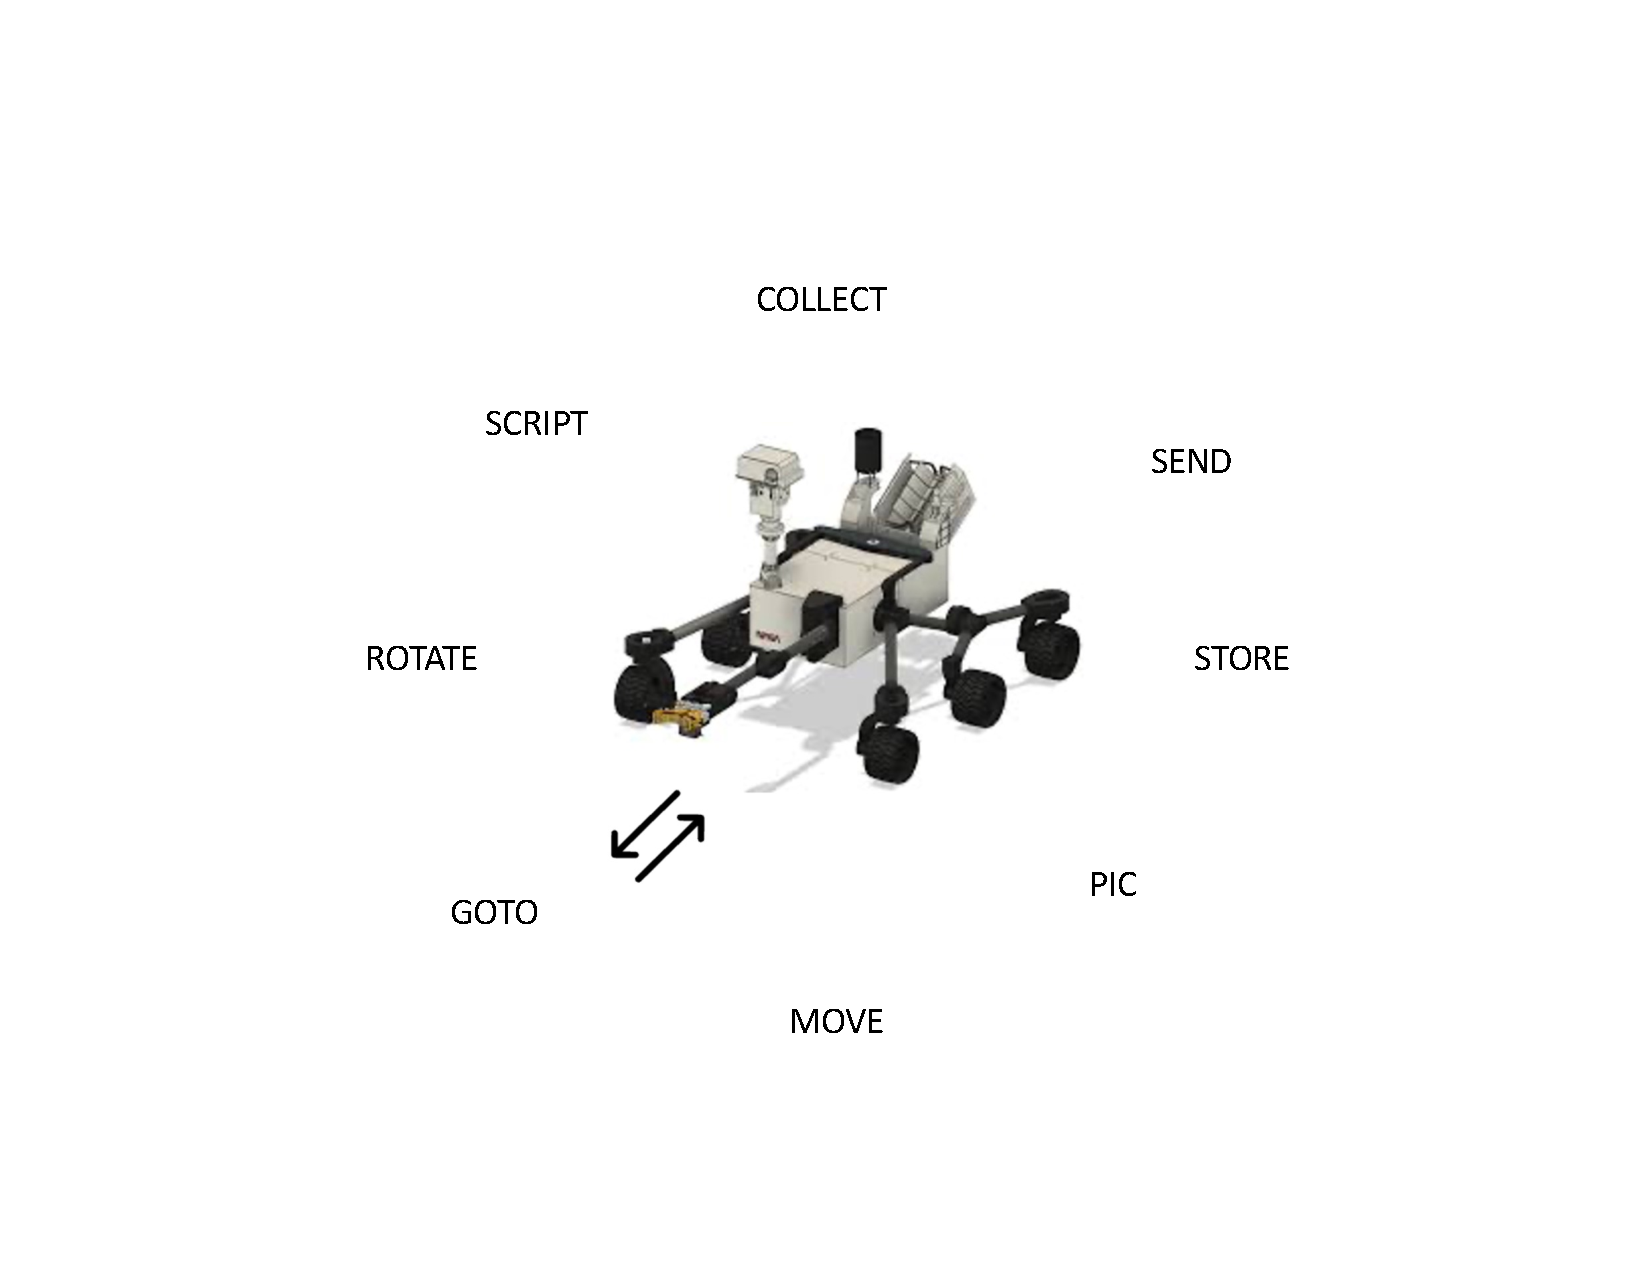
\includegraphics[width=1.0\textwidth]{figures/rover-actions.pdf}
%\caption{Your caption}
\end{figure}

\end{frame}


%----------------------------------------
\begin{frame}
  \frametitle{Rover example - commands} \small

{\scriptsize
\begin{center}
\texttt{direction} = \{ \texttt{forward},\ \texttt{backward} \} \\[0.5ex]
\texttt{image\_quality} = \{ \texttt{low},\ \texttt{medium},\ \texttt{high} \}
\end{center}
}

{\scriptsize
\[
\begin{array}{l}
\texttt{ROTATE}(number\!:\!\texttt{uint},\ time\!:\!\texttt{uint},\ angle\!:\!\texttt{float}) \\
\quad \text{where } -180 \le \texttt{angle} \le 180 \\ \\[0.5ex]
%
\texttt{GOTO}(number\!:\!\texttt{uint},\ time\!:\!\texttt{uint},\ x\!:\!\texttt{float},\ y\!:\!\texttt{float}) \\
\quad \text{where } -10000 \le \texttt{x,y} \le 10000 \\ \\[0.5ex]
%
\texttt{MOVE}(number\!:\!\texttt{uint},\ time\!:\!\texttt{uint},\ dir\!:\!\texttt{direction},\ distance\!:\!\texttt{float}) \\
\quad \text{where } 1 \le \texttt{distance} \le 1000 \\ \\[0.5ex]
%
\texttt{PIC}(number\!:\!\texttt{uint},\ time\!:\!\texttt{uint},\ quality\!:\!\texttt{image\_quality},\ images\!:\!\texttt{uint}) \\
\quad \text{where } 1 \le \texttt{images} \le 10 \\ \\[0.5ex]
%
\texttt{STORE}(number\!:\!\texttt{uint},\ time\!:\!\texttt{uint},\ file\!:\!\texttt{string},\ images\!:\!\texttt{uint}) \\
\quad \text{where } 1 \le \texttt{images} \le 10 \\ \\[0.5ex]
%
\texttt{SEND}(number\!:\!\texttt{uint},\ time\!:\!\texttt{uint},\ file\!:\!\texttt{string}) \\ \\[0.5ex]
%
\texttt{COLLECT}(number\!:\!\texttt{uint},\ time\!:\!\texttt{uint},\ file\!:\!\texttt{string},\ sample\!:\!\texttt{string}) \\ \\[0.5ex]
%
\texttt{SCRIPT}(number\!:\!\texttt{uint},\ time\!:\!\texttt{uint},\ script\!:\!\texttt{string},\ file\!:\!\texttt{string}) \\[0.5ex]
\end{array}
\]
}

\end{frame}

%----------------------------------------
\begin{frame}
  \frametitle{XML representation of commands} \scriptsize

\begin{figure}
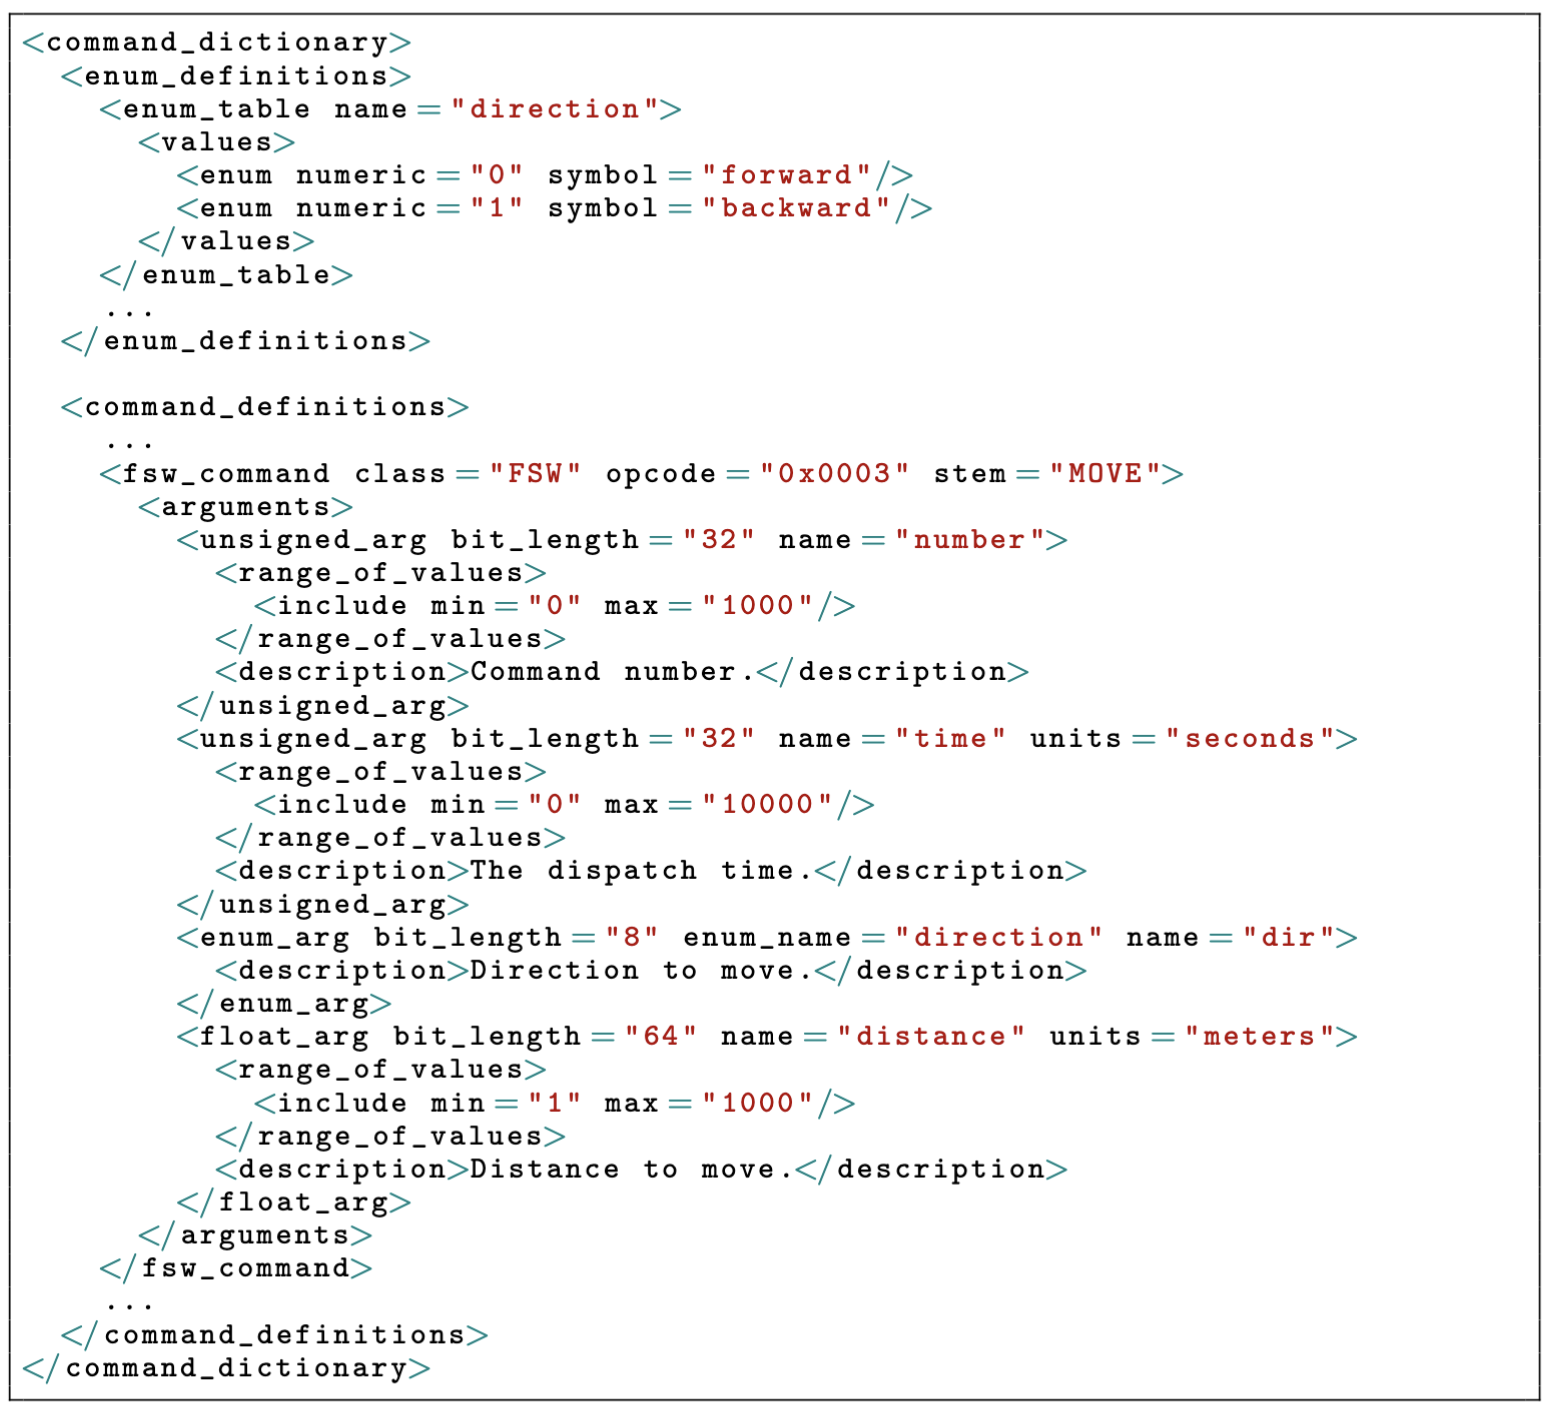
\includegraphics[width=0.71\textwidth]{figures/xml-commands.png}
%\caption{Your caption}
\end{figure}

\end{frame}


%----------------------------------------
\begin{frame}[fragile]
  \frametitle{Activating fuzz in Python} \small

% Types

% \begin{lstlisting}[language=python,frame=single]
% Command = Dict[str, Union[int, float, str]]
% Test = list[Command]

% \end{lstlisting}

% \pause

API

\begin{lstlisting}[language=python,frame=single]
def generate_tests(spec: Optional[str] = None, 
                   test_suite_size: Optional[int] = None, 
                   test_size: Optional[int] = None) -> list[Test]:
\end{lstlisting}

%\pause

% Configuration file used for default values

% \begin{lstlisting}[language=json]
% {
%     "cmd_files": ["xml/rover_commands.xml"],
%     "spec_file": "spec.txt",
%     "test_suite_size": 10,
%     "test_size": 10
% }
% \end{lstlisting}

\end{frame}

%----------------------------------------
\begin{frame}[fragile]
  \frametitle{Call fuzz without any constraints} \small

\begin{lstlisting}[language=python,frame=single]
from fuzz import generate_tests

tests = generate_tests(spec='', test_suite_size=100, test_size=10)
for test in tests:
    for cmd in test:
        print(cmd)
\end{lstlisting}

\pause

Yields a test of unconstrained random commands

\begin{lstlisting}[language=python,frame=single]
{'name': 'ROTATE', 'number': 51, 'time': 944, 'angle': -150.42}
{'name': 'SCRIPT', 'number': 75, 'time': 287, 'script': '...', 'file': '...'}
{'name': 'PIC', 'number': 64, 'time': 491, 'quality': 'low', 'images': 8}
{'name': 'SCRIPT', 'number': 48, 'time': 598, 'script': '...', 'file': '...'}
{'name': 'COLLECT', 'number': 39, 'time': 583, 'file': '...','sample': '...'}
{'name': 'COLLECT', 'number': 89, 'time': 78, 'file': '...', 'sample': '...'}
{'name': 'ROTATE', 'number': 87, 'time': 28, 'angle': 76.22}
{'name': 'GOTO', 'number': 90, 'time': 2, 'x': -8132.07, 'y': 4708.92}
{'name': 'PIC', 'number': 58, 'time': 531, 'quality': 'high', 'images': 6}
{'name': 'STORE', 'number': 74, 'time': 981, 'file': '...', 'images': 3}  
\end{lstlisting}

\end{frame}


%----------------------------------------
\begin{frame}[fragile]
  \frametitle{Defining constraints on all (any) commands} \small

\begin{block}{Requirements}
\begin{enumerate}
    \item Time must progress with steps no less than 10.
    \item Command numbers must increase by 1.
\end{enumerate}
\end{block}

\begin{lstlisting}[language=fuzzdsl,frame=single]
  rule p1: 
    always [any(time=t1?)] wnext [any(time=t2?)] t2 >= t1 + 10

  rule p2: 
    any(number=1) 
    and
    always [any(number=n1?)] wnext [any(number=n2?)] n2 = n1 + 1
\end{lstlisting}

\end{frame}


%----------------------------------------
\begin{frame}[fragile]
  \frametitle{Defining constraints on command arguments} \small

\begin{block}{Requirements}
\begin{enumerate}
    \setcounter{enumi}{2}
    \item The angle argument to ROTATE must be between -90 and 90.
    \item The distance argument to MOVE must be 1, 2 or 3.
\end{enumerate}
\end{block}

\begin{lstlisting}[language=fuzzdsl,frame=single]
  rule p3:   
    always [ROTATE(angle=a?)] -90 <= a <= 90
    
  rule p4: 
    always [MOVE(distance=d?)] (d = 1 or d = 2 or d = 3)   
\end{lstlisting}

\end{frame}


%----------------------------------------
\begin{frame}[fragile]
  \frametitle{Defining constraints on the future} \small

\begin{block}{Requirements}
\begin{enumerate}
\setcounter{enumi}{4}
\item  A MOVE command going backward, with a distance 'd', must be later followed be a ROTATE command, 
rotating with an angle 'a' satisfying $(d \le 1 \wedge a = 45) \vee (d > 1 \wedge a = 20)$.
\item Every GOTO command must be followed only by GOTO commands that move ``northeast'' (increasing in both x and y).
\end{enumerate}
\end{block}

\begin{lstlisting}[language=fuzzdsl,frame=single]
  rule p5: 
    always [MOVE(dir=direction.backwards,distance=d?)] 
      eventually <<ROTATE(angle=a?)>> 
                     ((d <= 1 and a = 45) or (d > 1 and a = 20))

  rule p6: 
    always [GOTO(x=x1?,y=y1?)] 
      always [GOTO(x=x2?,y=y2?)]  
        (x2 > x1 and y2 > y1)    
\end{lstlisting}

\end{frame}


%----------------------------------------
\begin{frame}[fragile]
  \frametitle{Defining constraints on strings with regular expressions} \small

\begin{block}{Requirements}
\begin{enumerate}
\setcounter{enumi}{6}
\item  if '$i$' high quality images are taken, then eventually a subset '$j$' ($0 < j \le i$)
of those images must be stored in a file with a name matching the regular
expression \verb+\d\d\d.img+ (e.g. {\tt 134.img}), and after that, this file must be sent to
the orbiting satellite.
\end{enumerate}
\end{block}

\begin{lstlisting}[language=fuzzdsl,frame=single]
  rule p7: 
    always [PIC(quality=image_quality.high, images=i?)]
      eventually <<STORE(file=f?, images=j?)>>
        (
          f |- /\d\d\d\.img/ 
          and
          0 < j <= i 
          and
          eventually SEND(file=f)
        ) 
\end{lstlisting}

\end{frame}


%----------------------------------------
\begin{frame}[fragile]
  \frametitle{Defining constraints about the past} \small

\begin{block}{Requirements}
\begin{enumerate}
\setcounter{enumi}{7}
\item If '$j$' images are stored in a file, then  
this file must not have been stored before, and also there must
have been taken a high quality picture in the past of a number of images '$i$'
($i \ge j$), and no file is stored since then except the current one.
\end{enumerate}
\end{block}

\begin{lstlisting}[language=fuzzdsl,frame=single]
  rule p8: 
    always [STORE(file=f?,images=j?)]
        prev ( 
          not once STORE(file=f) 
          and 
          (
            not STORE() 
            since 
            <<PIC(images=i?, quality=image_quality.high)>> i >= j
          )
        ) 
\end{lstlisting}

\end{frame}


%----------------------------------------
\begin{frame}[fragile]
  \frametitle{Defining constraints applying operations to data} \small

\begin{block}{Requirements}
\begin{enumerate}
\setcounter{enumi}{8}
\item If a sample collection named '$s$' is collected and the analysis result is stored in a
file '$f$', then later, without any other collection in
between, a script execution is commanded on that file '$f$',
where the script is named by concatenating \verb+"run_"+ with the sample name '$s$' 
and then \verb+".py"+.
\end{enumerate}
\end{block}

\begin{lstlisting}[language=fuzzdsl,frame=single]
  rule p9:     
    always [COLLECT(file=f?, sample=s?)] 
     next (
       not COLLECT()  
       until <<SCRIPT(script = k?, file=f)>> k = "run_" + s + ".py"
     )  
\end{lstlisting}

\end{frame}


%----------------------------------------
\begin{frame}[fragile]
  \frametitle{Defining constraints forcing commands to occur} \small

\begin{block}{Requirements}
\begin{enumerate}
\setcounter{enumi}{9}
\item We want to see a MOVE, a PIC with high image quality, 
and a COLLECT command.
\end{enumerate}
\end{block}

\begin{lstlisting}[language=fuzzdsl,frame=single]
  rule p10: 
    eventually MOVE() and 
    eventually PIC(quality=image_quality.high) and 
    eventually COLLECT()
\end{lstlisting}

\end{frame}


%----------------------------------------
\begin{frame}[fragile]
  \frametitle{Applying fuzz with our constraints} \small

We can now call \ipyt{generate_tests} with this specification
as follows:

\begin{lstlisting}[language=python,frame=single]
spec = """
  rule p1:  ...
  ...
  rule p10: ...
"""

tests = generate_tests(spec=spec, test_suite_size=100, test_size=10)

# ... process tests ...
\end{lstlisting}

\end{frame}


%----------------------------------------
\begin{frame}[fragile]
  \frametitle{Example of a generated constrained test} \small

This test satisfies all 10 properties.

\begin{lstlisting}[language=python]
{'name': 'SCRIPT', 'number': 1, 'time': 1, 'script': '...', 'file': '...'}
{'name': 'PIC', 'number': 2, 'time': 11, 'quality': 'high', 'images': 10}
{'name': 'STORE', 'number': 3, 'time': 21, 'file': '...', 'images': 8}
{'name': 'SEND', 'number': 4, 'time': 31, 'file': '...'}
{'name': 'MOVE', 'number': 5, 'time': 41, 'dir': 'forward', 'distance': 1.0}
{'name': 'PIC', 'number': 6, 'time': 51, 'quality': 'high', 'images': 10}
{'name': 'STORE', 'number': 7, 'time': 61, 'file': '482.img', 'images': 7}
{'name': 'COLLECT', 'number': 8, 'time': 71, 'file': 'm', 'sample': 'm'}
{'name': 'SCRIPT', 'number': 9, 'time': 81, 'script': 'run_m.py', 'file':'m'}
{'name': 'SEND', 'number': 10, 'time': 91, 'file': '482.img'}    
\end{lstlisting}

% \pause

% \begin{block}{Execution time}
% \begin{itemize}
% \item 100 tests generated in 38 minutes, 23 seconds per test. 
% \pause
% \underline{Culprit: the regular expression match}
% \ifuzz{f |- /\d\d\d\.img/} in rule \ifuzz{p7}.

% \pause

% \item 100 tests generated in 68 seconds, 0.7 seconds per test, \underline{if we remove that 
% regular expression string constraint}.
% \end{itemize}
% \end{block}

% In general, string operations can be costly when using an SMT constraint solver.

\end{frame}



%----------------------------------------
\begin{frame}<0>[fragile]
  \frametitle{A mini SMT lecture} \small

\begin{block}{SMT problem: constraint on an integer variable}
\[
\begin{aligned}
& x : \intg \\
& x > 10
\end{aligned}
\]
\end{block}

\pause

\[
[x \mapsto 11]
\]

\pause

\begin{block}{SMT problem: constraint on a function}
\[
\begin{aligned}
& f : \mathbb{Z} \to \mathbb{Z} \\
& \forall x, y \in \mathbb{Z},\ f(x) = f(y) \Rightarrow x = y
\end{aligned}
\]
\end{block}

\pause

\[
[f \mapsto \lambda x. x]
\]

\end{frame}


%----------------------------------------
\begin{frame}<0>[fragile]
  \frametitle{Constraint on a function in SMT-LIB} \small

\begin{block}{SMT problem: constraint on a function}
\begin{verbatim}
    (declare-fun f (Int) Int)
    (assert
      (forall ((x Int) (y Int))
        (=> (= (f x) (f y)) (= x y))
      )
    )
\end{verbatim}
\end{block}

\begin{verbatim}
    sat
    (model
      (define-fun f ((x Int)) Int
        x)
    )
\end{verbatim}

\end{frame}


%----------------------------------------
\begin{frame}<0>[fragile]
  \frametitle{Representing a test as a function from time to commands} \small

{\bf The SMT type of tests:}

\begin{lstlisting}[language=python,frame=single]
test: Function = Function('test', IntSort(), Command)
\end{lstlisting}

\pause

{\bf The SMT type of commands:}

{\scriptsize
\begin{verbatim}
(declare-datatypes ()
  (
    (Command
      (ROTATE (ROTATE_number Int)(ROTATE_time Int)(ROTATE_angle Real))
      (GOTO (GOTO_number Int)(GOTO_time Int)(GOTO_x Real)(GOTO_y Real))
      (MOVE (MOVE_number Int)(MOVE_time Int)
            (MOVE_dir direction)(MOVE_distance Real))
      (PIC (PIC_number Int)(PIC_time Int)
           (PIC_quality image_quality)(PIC_images Int))
      (STORE (STORE_number Int)(STORE_time Int)
             (STORE_file String)(STORE_images Int))
      (SEND (SEND_number Int)(SEND_time Int)(SEND_file String))
      (COLLECT (COLLECT_number Int)(COLLECT_time Int)
               (COLLECT_file String)(COLLECT_sample String))
      (SCRIPT (SCRIPT_number Int)(SCRIPT_time Int)
              (SCRIPT_script String)(SCRIPT_file String))
    )
  )
)    
\end{verbatim}
}

\end{frame}


%----------------------------------------
\begin{frame}<0>[fragile]
  \frametitle{Modeling temporal logic in first-order logic on a finite trace} \small

{\bf Consider the \underline{propositional} temporal formula:} $\Box (p \rightarrow \Diamond q)$

\pause

\vspace{0.2cm}
{\bf One can model it in first-order logic with quantifiers:}

\[
\forall i \in \{0..k\!-\!1\},\ p(test(i)) 
  \rightarrow 
    \exists j \in \{i..k\!-\!1\}, q(test(j)))
\]

\pause

\vspace{0.2cm}
{\bf For efficiency we instead ``unfold'' the quantifiers (here for trace length 3):} 

\begin{align*}
&p(test(0)) \rightarrow (q(test(0)) \vee q(test(1)) \vee q(test(2))) \\
\wedge\quad &p(test(1)) \rightarrow (q(test(1)) \vee q(test(2))) \\
\wedge\quad &p(test(2)) \rightarrow q(test(2))
\end{align*}

\pause

\vspace{0.2cm}
{\bf And a rewrite, recalling that $p \rightarrow q \equiv \neg p \vee q$:}

\begin{align*}
&\neg p(test(0)) \vee q(test(0)) \vee q(test(1)) \vee q(test(2)) \\
\wedge\quad &\neg p(test(1)) \vee q(test(1)) \vee q(test(2)) \\
\wedge\quad &\neg p(test(2)) \vee q(test(2))
\end{align*}

\end{frame}


%----------------------------------------
\newcommand{\isM}[1]{\mathtt{isM}(#1)}
\newcommand{\isR}[1]{\mathtt{isR}(#1)}
\newcommand{\Mdir}[1]{\mathtt{Mdir}(#1)}
\newcommand{\Mdist}[1]{\mathtt{Mdist}(#1)}
\newcommand{\Rangle}[1]{\mathtt{Rangle}(#1)}

\begin{frame}<0>[fragile]
  \frametitle{Let's now look at the more complicated property p5} \small

\begin{lstlisting}[language=fuzzdsl,frame=single]
  rule p5: # a backward move leads to a future rotation
    always [MOVE(dir=direction.backwards,distance=d?)] 
      eventually <<ROTATE(angle=a?)>> 
                     ((d <= 1 and a = 45) or (d > 1 and a = 20))  
\end{lstlisting}

\pause

\vspace{-0.3cm}

First we define some shorthands:
\hfill
\begin{minipage}{0.55\linewidth}
{\scriptsize
\begin{align*}
\isM{i}    &= \mathsf{is}(\mathsf{MOVE}, \mathsf{test}(i)) \\
\isR{i}    &= \mathsf{is}(\mathsf{ROTATE}, \mathsf{test}(i)) \\
\Mdir{i}   &= \mathsf{MOVE\_dir}(\mathsf{test}(i)) \\
\Mdist{i}  &= \mathsf{MOVE\_distance}(\mathsf{test}(i)) \\
\Rangle{i} &= \mathsf{ROTATE\_angle}(\mathsf{test}(i)) \\
\end{align*}
}
\end{minipage}

\pause

\vspace{-0.3cm}

\begin{block}{The SMT formula generated}
{\scriptsize
\[
\begin{aligned}
\bigwedge_{i=0}^{n-1} \Bigl(
   & \neg\bigl(\isM{i} \wedge \Mdir{i}=backward\bigr) \\[0.5ex]
   & \;\;\vee\;
     \bigvee_{j=i}^{n-1} \Bigl(
        \isR{j} \wedge
        \bigl(
           (\Mdist{i}\le 1 \wedge \Rangle{j}=45) 
           \vee\;
           (\Mdist{i} > 1 \wedge \Rangle{j}=20)
        \bigr)
     \Bigr)
\Bigr)
\end{aligned}
\]
}
\end{block}

\end{frame}

%----------------------------------------
\begin{frame}<0>[fragile]
  \frametitle{Show me the code} \small

\begin{block}{The until formula}
\[
\varphi_1 \until \varphi_2
\]
\end{block}

\begin{lstlisting}[language=python,frame=single]
@dataclass
class LTLUntil(LTLFormula):
  left: LTLFormula
  right: LTLFormula

  def to_smt(self, env: Environment, t: int, end_time: int) -> BoolRef: ...

  def evaluate(self, env: Environment, test: Test, index: int) -> bool: ...
\end{lstlisting}

\end{frame}


%----------------------------------------
\begin{frame}<0>[fragile]
  \frametitle{The to\_smt method} \small

\begin{block}{Follows this expansion approach}
\[
\varphi_1 \until \varphi_2 = 
  \varphi_2(0) 
  \vee (\varphi_2(1) \wedge \varphi_1(0))  
  \vee (\varphi_2(2) \wedge \varphi_1(0) \wedge \varphi_1(1))
  \vee ...
\]
\end{block}

\begin{lstlisting}[language=python,frame=single]
@dataclass
class LTLUntil(LTLFormula):
  left: LTLFormula
  right: LTLFormula

  def to_smt(self, env: Environment, t: int, end_time: int) -> BoolRef:
    return Or(
      [
        And(
          self.right.to_smt(env, t_prime, end_time),
          And([self.left.to_smt(env, t_i, end_time) 
                for t_i in range(t, t_prime)])
        )
        for t_prime in range(t, end_time)
      ])
\end{lstlisting}

\end{frame}


%----------------------------------------
\begin{frame}<0>[fragile]
  \frametitle{The evaluate method} \small

\begin{block}{Follows the semantics}
% \[
% (\gamma,\sigma,j) \models \varphi_2 \;\text{{\bf for some}}\; i \leq j < |\sigma|
% \;\text{{\bf and for all}}\; i \le k < j: \; (\gamma,\sigma,k) \models \varphi_1
% \]

\[
\varphi_1 \until \varphi_2 = \varphi_2 \vee (\varphi_1 \wedge \Next (\varphi_1 \until \varphi_2))
\]
\end{block}

\begin{lstlisting}[language=python,frame=single]
@dataclass
class LTLUntil(LTLFormula):
  left: LTLFormula
  right: LTLFormula

  def evaluate(self, env: Environment, test: Test, index: int) -> bool:
    if within(index, test):
      return self.right.evaluate(env, test, index) or (
        self.left.evaluate(env, test, index) 
          and 
        self.evaluate(env, test, index + 1)
      )
    return False
\end{lstlisting}

\pause

Since $\Diamond \varphi = \true \until \varphi\tt$ one can easily see that
the temporal formula $\Diamond \varphi$ will generate an SMT formula of the form 
$\varphi(0)  \vee \varphi(1) \vee \varphi(2)  \vee ... \vee \varphi(k-1)$.


\end{frame}


%----------------------------------------
\begin{frame}<0>[fragile]
  \frametitle{But SMT solvers are not random enough} \small

\begin{block}{Consider our first two formulas}
\begin{lstlisting}[language=fuzzdsl,frame=single]
  rule p1: 
    always [any(time=t1?)] wnext [any(time=t2?)] t2 >= t1 + 10

  rule p2: 
    any(number=1) 
    and
    always [any(number=n1?)] wnext [any(number=n2?)] n2 = n1 + 1
\end{lstlisting}
\end{block}

\pause
Z3 may return the following test:

\begin{lstlisting}[language=python]
{'name': 'SCRIPT', 'number': 1, 'time': 363, 'script': '', 'file': ''}
{'name': 'SCRIPT', 'number': 2, 'time': 373, 'script': '', 'file': ''}
{'name': 'SCRIPT', 'number': 3, 'time': 383, 'script': '', 'file': ''}
{'name': 'SCRIPT', 'number': 4, 'time': 393, 'script': '', 'file': ''}
{'name': 'SCRIPT', 'number': 5, 'time': 403, 'script': '', 'file': ''}
\end{lstlisting}

with five SCRIPT commands!

\end{frame}


%----------------------------------------
\begin{frame}<0>[fragile]
  \frametitle{We need to further randomize the tests produced by Z3} \small

%\begin{algorithm}
\begin{algorithmic}[1]
\State \textbf{Input:} A \matl{} specification and a test satisfying the specification 
\State \textbf{Output:} A more randomized test still satisfying the specification
\For{each command $c$ in the test}
    \State Replace $c$ with a random command $c'$ 
    \If{the modified test satisfies the specification}
        \State Keep the replacement $c'$
    \Else
        \State Restore original command $c$
        \State \# {\em Randomize arguments:}
        \For{each argument $a$  of $c$} 
          \State Replace $a$ with a random argument $a'$
          \State \# {\em Test whether new argument works:}
          \If{the modified test satisfies the specification}
            \State Keep the replacement $a'$
          \Else
            \State Restore original argument $a$
          \EndIf
        \EndFor
    \EndIf
\EndFor
\State \Return randomized test
\end{algorithmic}
%\end{algorithm}

\end{frame}


%----------------------------------------
\begin{frame}<0>[fragile]
  \frametitle{After applying refinement a more random test is generated still satisfying the two constraints} \small

\begin{lstlisting}[language=python]
{'name': 'SEND', 'number': 1, 'time': 363, 'file': '...'}
{'name': 'SCRIPT', 'number': 2, 'time': 373, 'script': '...', 'file': '...'}
{'name': 'SEND', 'number': 3, 'time': 383, 'file': '...'}
{'name': 'COLLECT', 'number': 4, 'time': 393, 'file': '...', 'sample': '...'}
{'name': 'STORE', 'number': 5, 'time': 403, 'file': '...', 'images': 8}
\end{lstlisting}

Allthough time values increase exactly by 10.

\pause

\begin{block}{It is a heuristic}

\begin{itemize}

    \item A simpler version was tried that consisted of not including lines 10-18 that randomize arguments. This solution was less effective. 
    
    \item Another tried solution consisted, instead of lines 5-19, of invoking the SMT solver repeatedly with new random commands, and if it succeeded in generating a new test, the new command was kept. However, this did not scale well.

\end{itemize}

\end{block}

\end{frame}




%
%----------------------------------------
\begin{frame}[fragile]
  \frametitle{Evaluation - strings are costly} \small

\begin{figure}
\centering
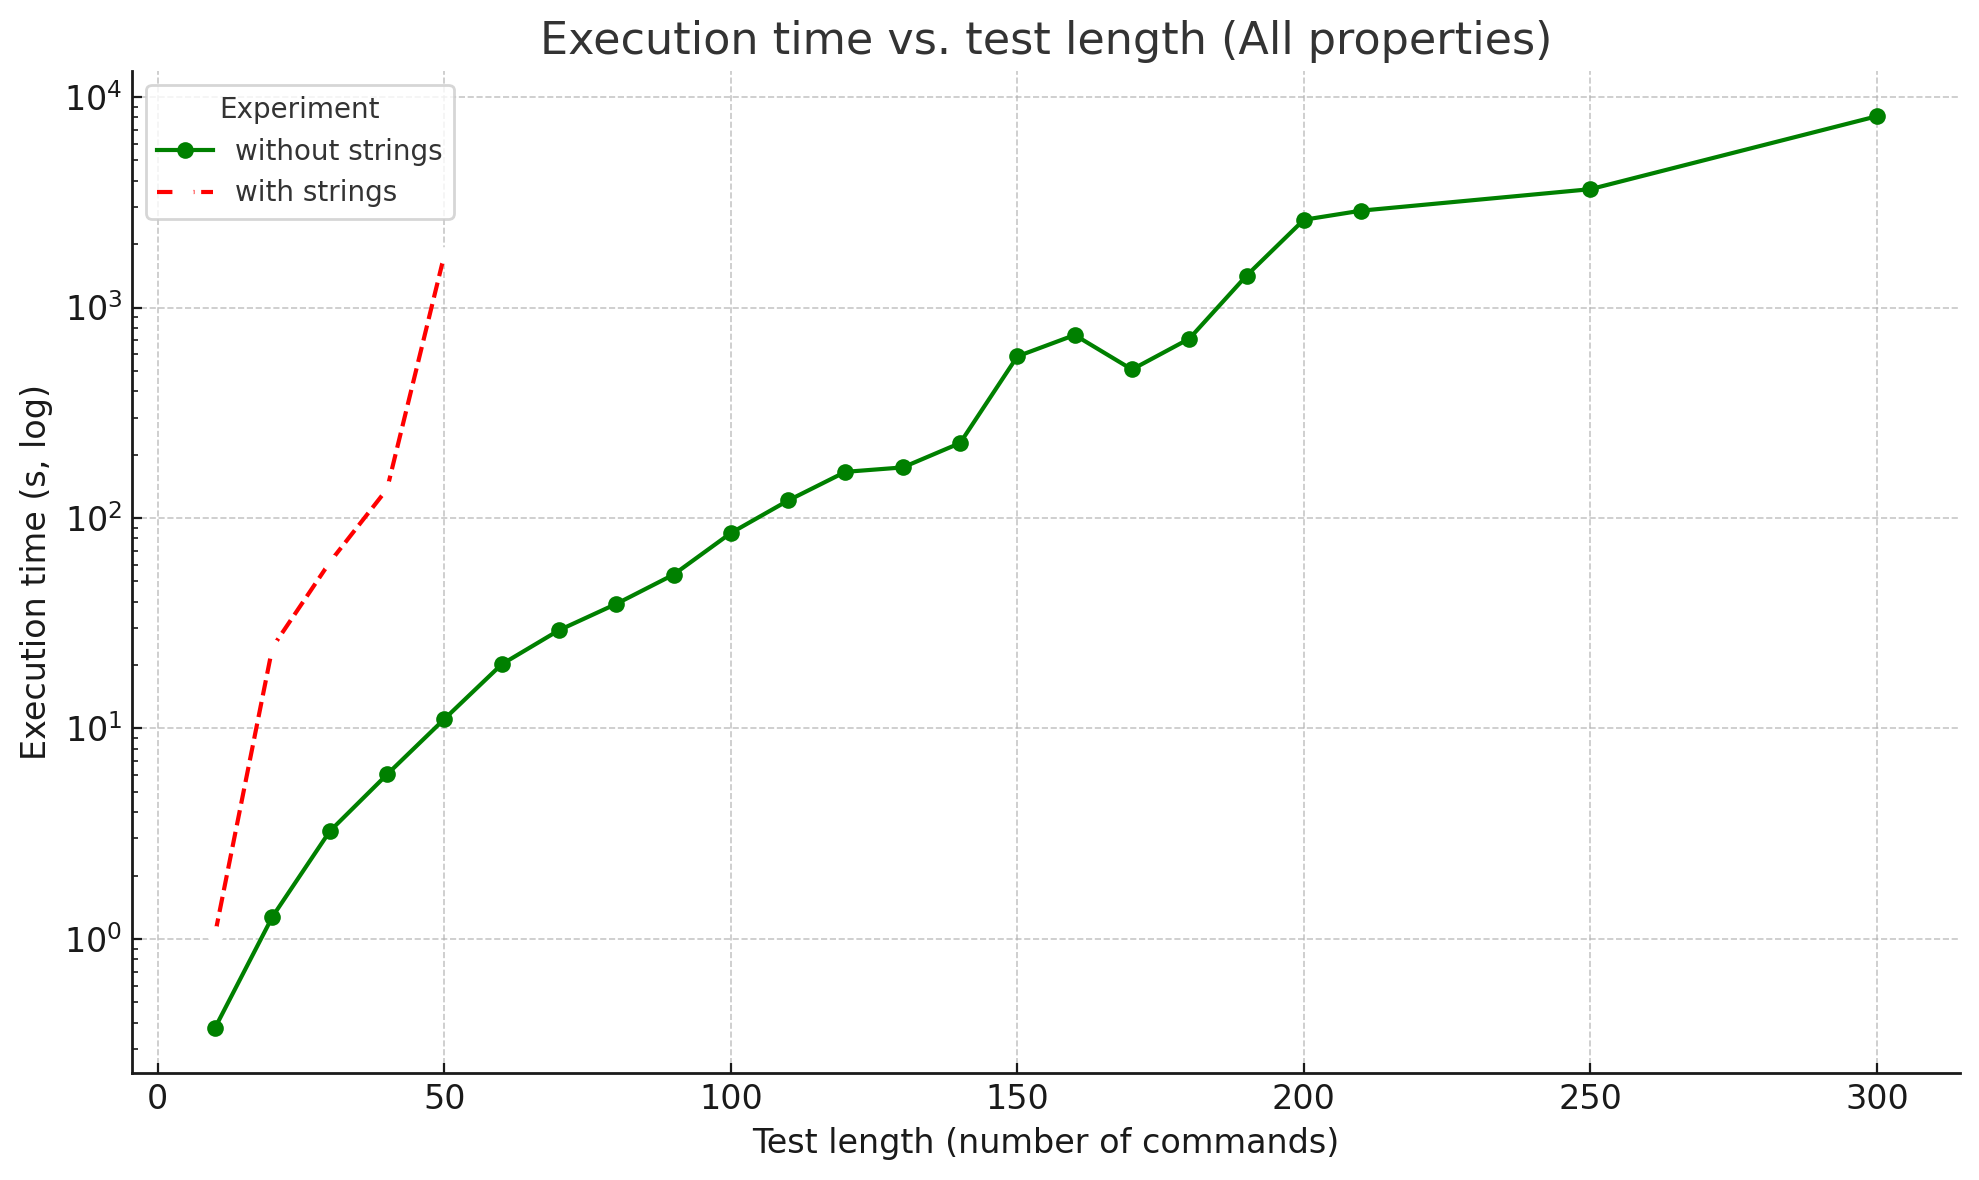
\includegraphics[width=.8\textwidth]{figures/graph-execution.png}
\caption{Execution times (log scale) for all properties combined.}
\end{figure}

\end{frame}


%----------------------------------------
\begin{frame}[fragile]
  \frametitle{Evaluation - strings are costly} \small

\begin{figure}[t]
\centering
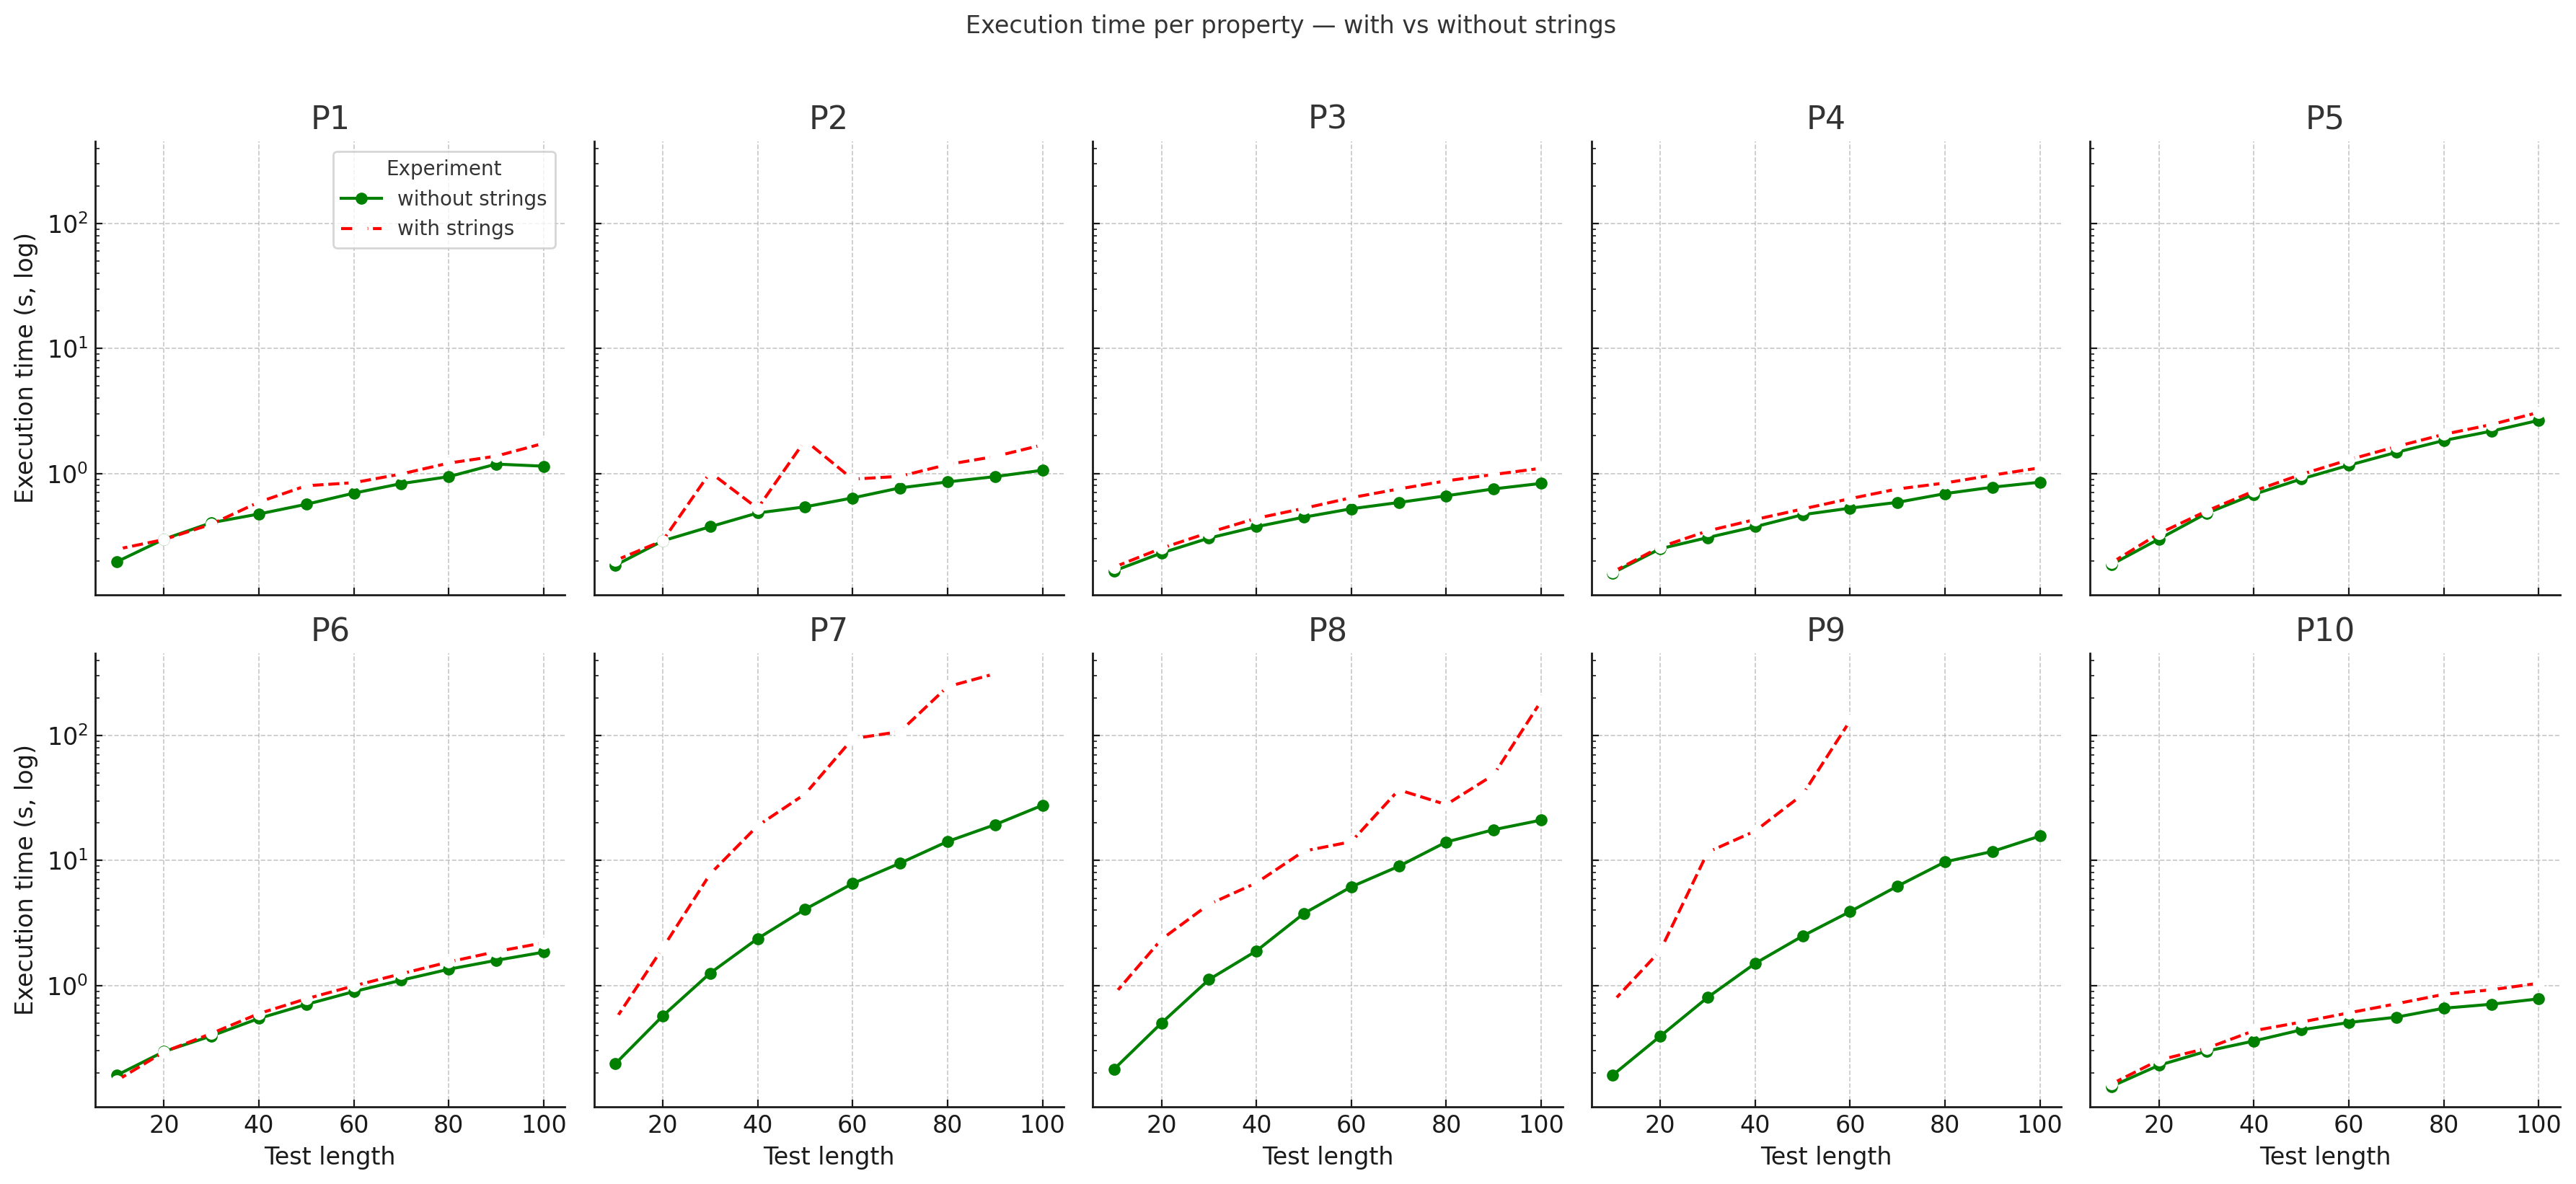
\includegraphics[width=.8\textwidth]{figures/graph-per-property.png}
\caption{Execution times (log scale) per property.}
\end{figure}

\end{frame}


%----------------------------------------
\begin{frame}[fragile]
  \frametitle{Second application}

{\Large\bf Using Temporal Constraints to Generate Schedules}

\end{frame}

%----------------------------------------
\begin{frame}[fragile]
  \frametitle{Inspiration: the MEXEC scheduling system}

\begin{figure}
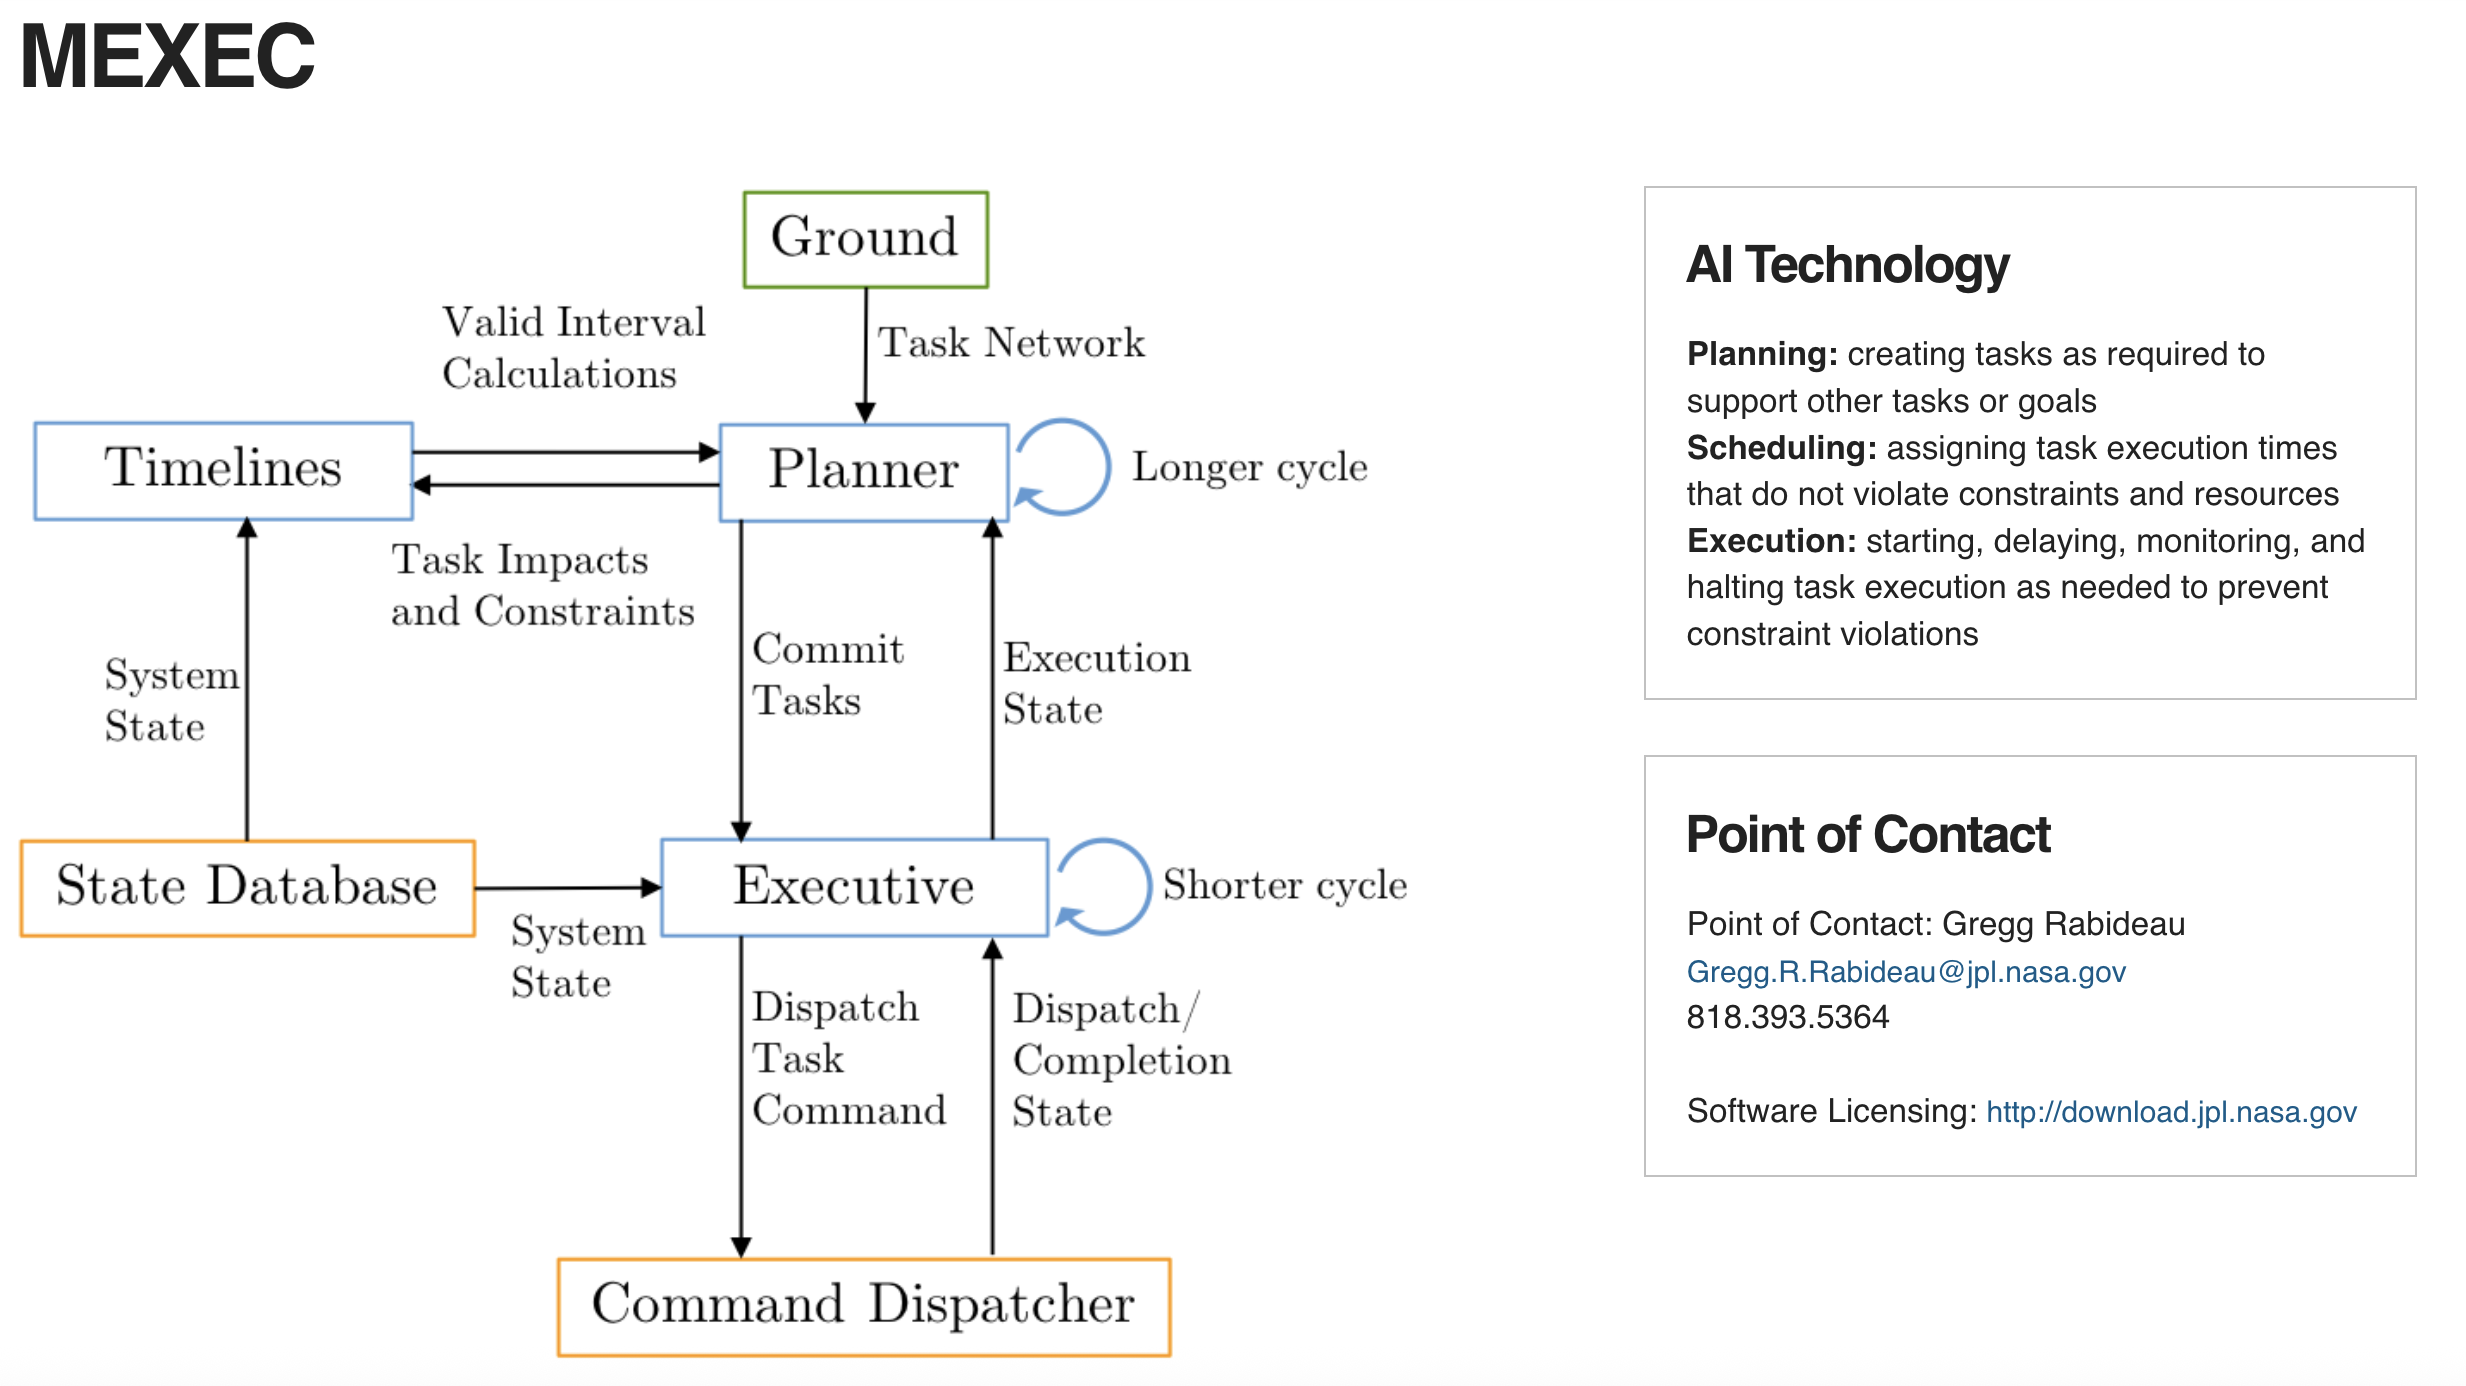
\includegraphics[width=1.0\textwidth]{figures/mexec.png}
%\caption{Your caption}
\end{figure}

\end{frame}

%----------------------------------------
\begin{frame}[fragile]
  \frametitle{A tasknet: timelines} \small

\begin{lstlisting}[language=tasknetdsl,frame=single]
tasknet Rover {
  end = 400;

  timelines {
    arm : atomic = false;
    location : state(home, target) = home;
    data : cumulative [0.0, 50.0] bounds [0.0, 100.0] = 0.0;
    battery : rate [10.0, 100.0] bounds [0.0, 100.0] = 60.0;
    temperature : rate [5.0, 40.0] bounds [0.0, 100.0] = 10.0;
  }

  task drive { ... }
  task collect { ... }
  optional task charge { ... }
  optional task heating { ... }
}
\end{lstlisting}

\end{frame}

%----------------------------------------
\begin{frame}[fragile]
  \frametitle{A tasknet: tasks} \small

\begin{lstlisting}[language=tasknetdsl,frame=single]
  task drive {
    startrange [100, 120];
    endrange [130, 160];
    durationrange [30,40];

    pre {
      battery in [60.0, 100.0]; 
      temperature in [10.0, 40.0]; 
    }

    impacts {
      maint {
        battery +~ -1.5;  
      }
      post {
        location = target;
      }
    }
  }
\end{lstlisting}

\end{frame}

%----------------------------------------
\begin{frame}[fragile]
  \frametitle{A tasknet: tasks} \small

\begin{lstlisting}[language=tasknetdsl,frame=single]
  task collect {
    durationrange  [20, 30];

    pre {
      location = target;
      battery in [60.0, 100.0];
      arm = false;
    }

    impacts {
      pre {
        arm = true;
      }
      maint {
        battery +~ -0.5; 
        temperature +~ -0.2;
      }
      post {
        data += 40.0; 
        arm = false;
      }
    }
  }
\end{lstlisting}

\end{frame}

%----------------------------------------
\begin{frame}[fragile]
  \frametitle{A tasknet: optional tasks} \small

\begin{lstlisting}[language=tasknetdsl,frame=single]
 optional task charge {
    durationrange [60,70];

    pre {
      battery in [0.0, 60.0];
    }

    impacts {
      maint {
        battery +~ 2.0; 
      }
    }
  }

  optional task heating {
    duration_range [10, 10];

    impacts {
      maint {
        battery +~ -0.5; 
        temperature +~ 2; 
      }
    }
  }  
\end{lstlisting}

\end{frame}

%----------------------------------------
\begin{frame}[fragile]
  \frametitle{A tasknet: temporal constraints and properties} \small

\begin{lstlisting}[language=tasknetdsl,frame=single]
  constraints {
    prop charge_drive:   always not (active(charge) and active(drive));
    prop temperature10:  always temperature >= 10;
  }
\end{lstlisting}

\pause

\begin{lstlisting}[language=tasknetdsl,frame=single]
  properties {
    prop target_reached: eventually (location = target and data >= 30);
    prop drive_charge:   always (active(drive) -> eventually active(charge));
    prop temperature:    always temperature >= 10;
  }
\end{lstlisting}

\end{frame}

%----------------------------------------
\begin{frame}[fragile]
  \frametitle{A generated schedule} \small

\begin{verbatim}
Schedule for TaskNet `Rover3`:
  drive         : start =  118, end =  148
  heating       : start =  137, end =  147
  charge        : start =  149, end =  209
  collect       : start =  210, end =  233

PROPERTY 'target_reached' HOLDS
PROPERTY 'drive_charge' HOLDS
PROPERTY 'temperature' HOLDS
\end{verbatim}

\end{frame}

%----------------------------------------
\begin{frame}[fragile]
  \frametitle{A Generated Schedule} \small

\begin{verbatim}
-- zone 1: (118, 137] --
    active tasks : drive
    arm            = False
    location       = home
    data           = 0
    battery        = 60 -> 31.5
    temperature    = 10 -> 10

  -- zone 2: (137, 147] --
    active tasks : drive, heating
    arm            = False
    location       = home
    data           = 0
    battery        = 31.5 -> 11.5
    temperature    = 10 -> 30
  ...
\end{verbatim}

\end{frame}

%----------------------------------------
\begin{frame}[fragile]
  \frametitle{The scheduling and the verification problem} \small

\begin{block}{The scheduling problem}
\[
\exists initial . \exists schedule . constraints(initial, schedule)
\]
\end{block}

\pause

\begin{block}{The verification problem, proving property $\varphi$ for all schedules}
\[
\forall initial . \forall schedule . constraints(initial, schedule) \rightarrow \varphi(schedule)
\]
\end{block}

\end{frame}

%----------------------------------------
\begin{frame}
  \frametitle{TaskSAT VS extension for syntax highlighting} \small

\begin{figure}
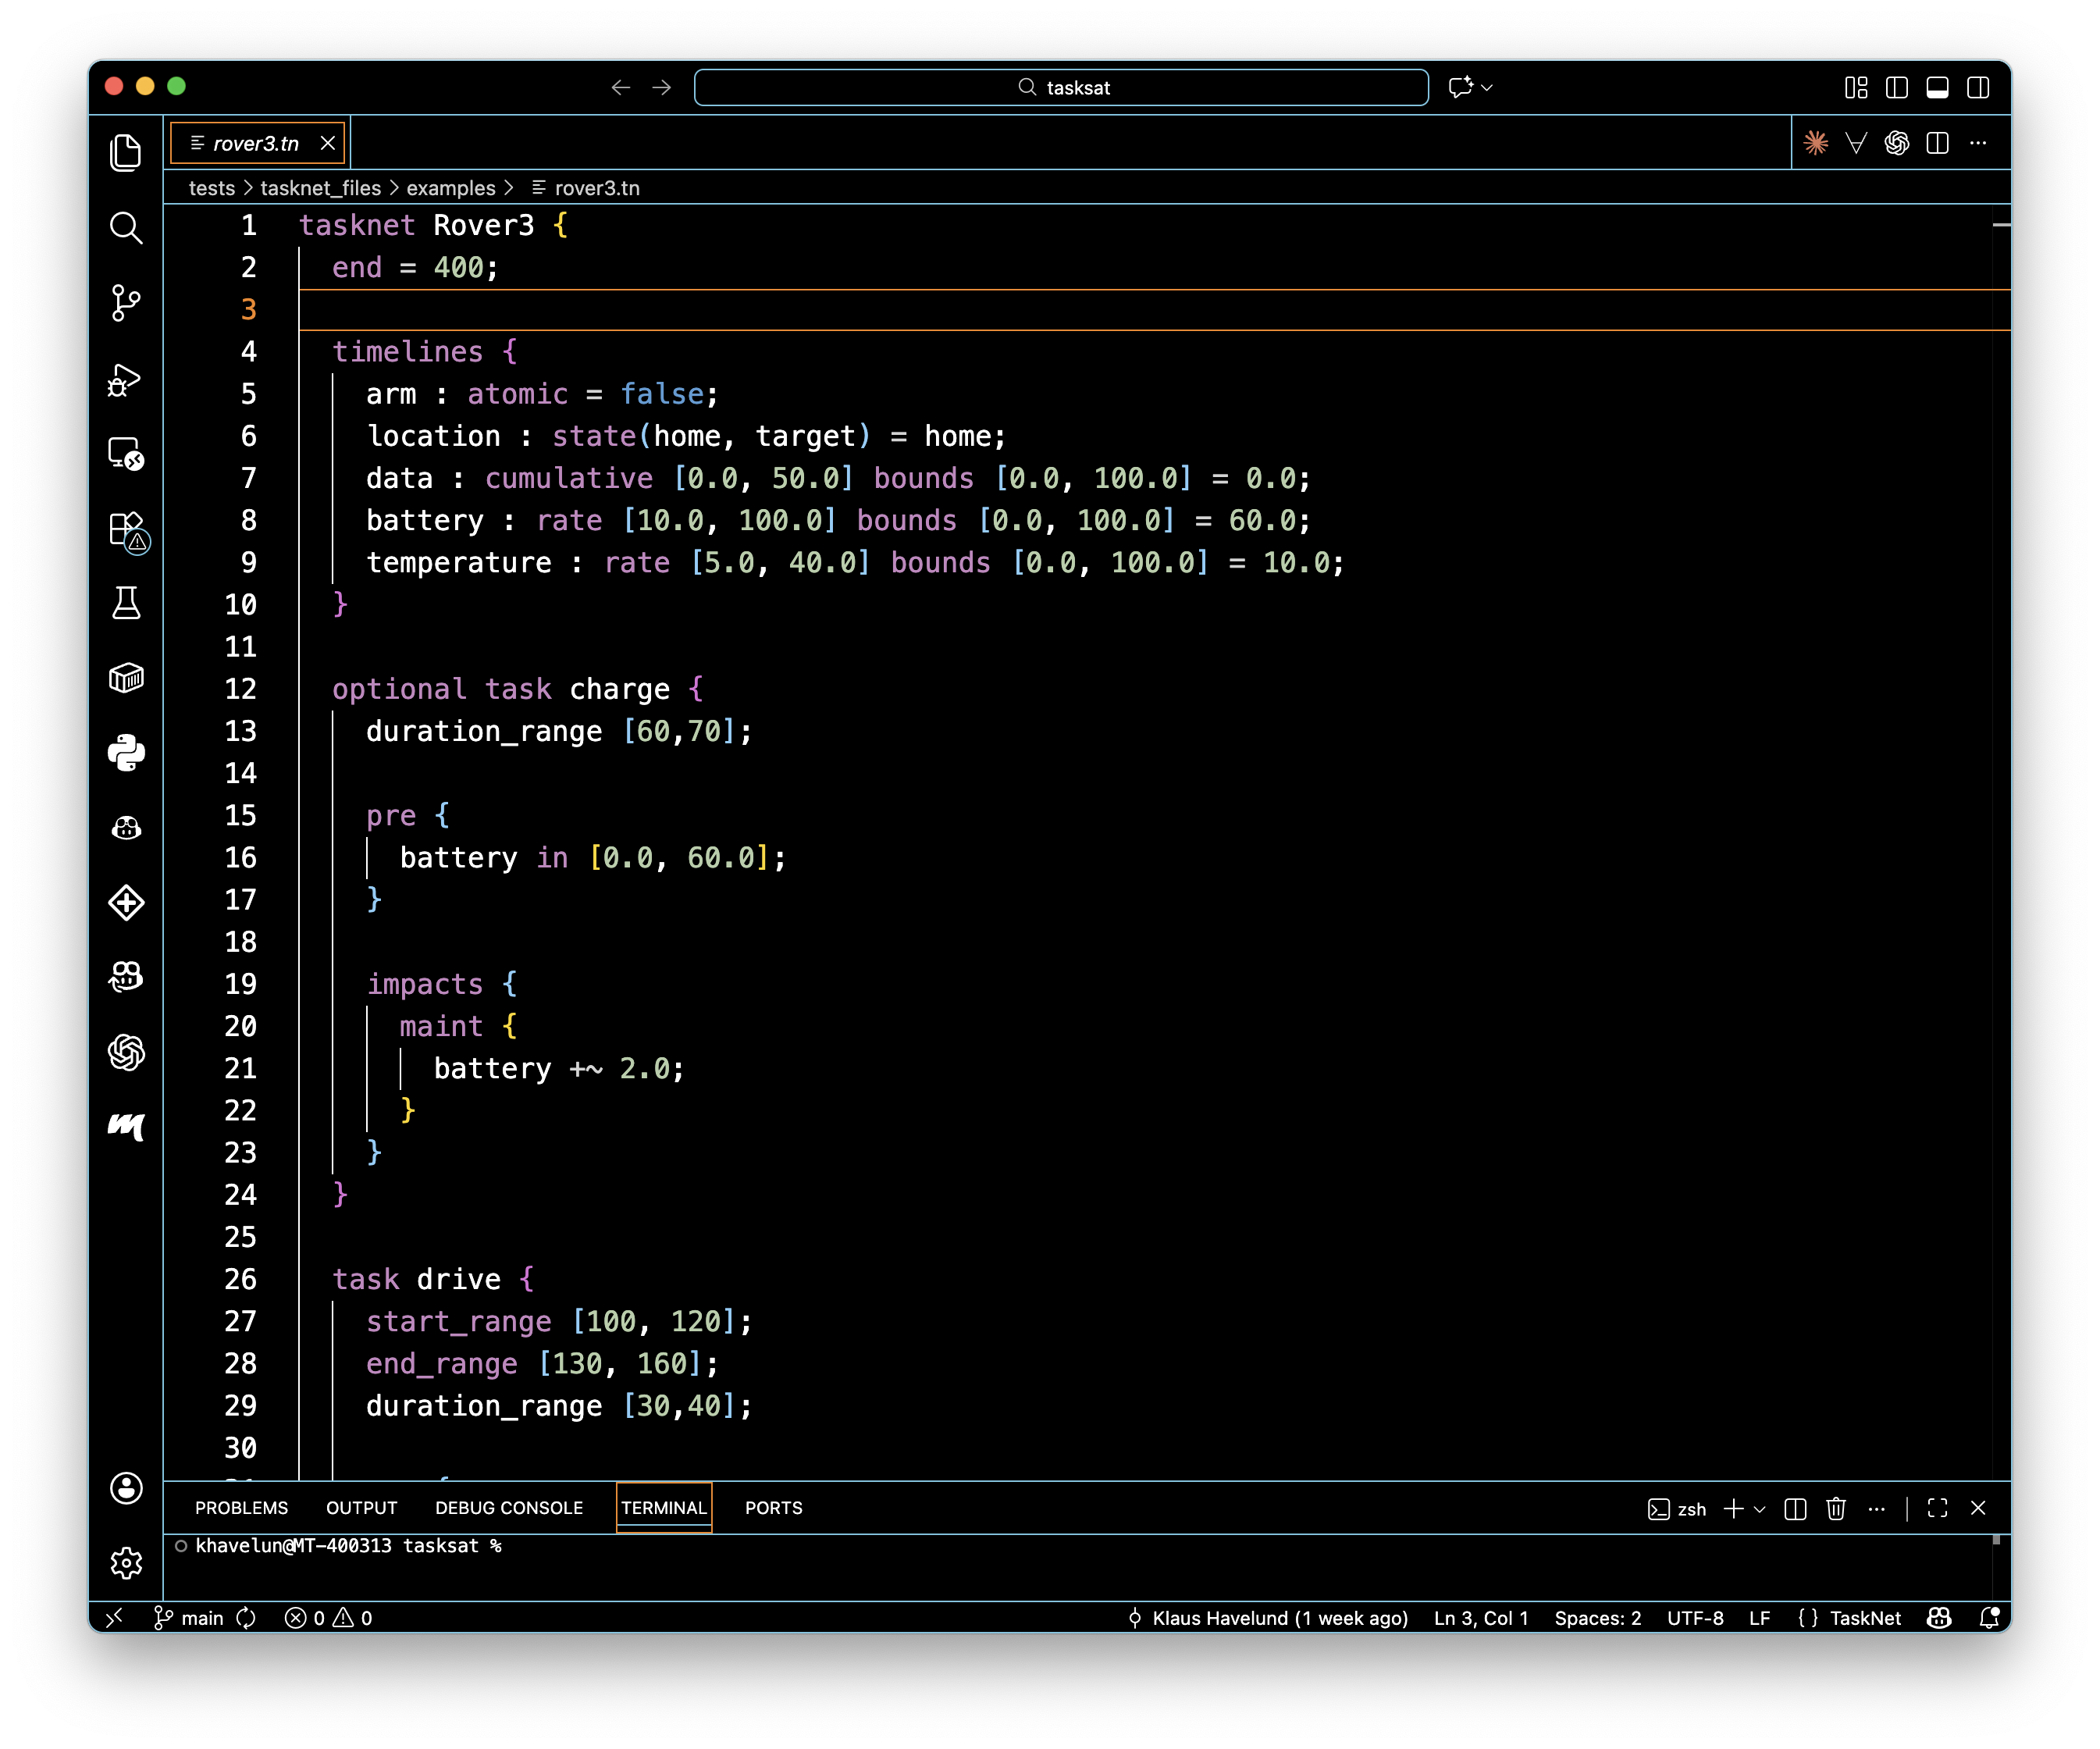
\includegraphics[width=0.85\textwidth]{figures/vs-code.png}
%\caption{Your caption}
\end{figure}

\end{frame}

%----------------------------------------
\begin{frame}[fragile]
  \frametitle{Conclusion} \small

\begin{itemize}

  \item Temporal logic can be a powerful formalism for expressing
  temporal constraints on sequences, here used to {\bf generate} sequences.

  \pause

  \item One can develop alternative (perhaps more userfriendly) formalisms
  for expressing temporal constraints, including e.g graphical formalisms.

  \pause

  \item Constraint solving using SMT solvers (such as Z3) is an efficient
  and automated way of generating sequences (tests, schedules, ...) satisfying temporal constraints.

  \pause

  \item Disclaimer: scalability can, as usual for these kinds of techniques, be an issue. 

  \pause

  \item Temporal properties can also be used to {\bf monitor} sequences. This is
  the field of {\em runtime verification}. That's another talk.

\end{itemize}

%\begin{block}{fuzz is available here}
%\begin{center}
%\url{https://github.com/havelund/fuzzing}
%\end{center}
%\end{block}

\end{frame}


\end{document}

